\documentclass{pnp_article}

\externaldocument{../pus/PusExtension}  % Allows cross-references to Def. Doc.
\externaldocument{../um/PusExtensionUM}   	% Allows cross-references to UM

\begin{document}

\SetDocIssue{0.2}
\SetDocRefNumber{PP-RP-PUX-0001}
\SetDocTitle{CORDET Framework - PUS Extension}
\SetDocSubtitle{Software Verification Report}
\SetDocAuthor{Alessandro Pasetti}
\SetCheckedBy{n.a.}
\maketitle

\maketitle

\newpage
\tableofcontents
%\newpage
%\listoffigures
%\newpage
%\listoftables

%---------------------------------------------
% Import file with definition of commands and reports
%---------------------------------------------
\def \printOutCmpVerSuccAccRepSpec#1 {
\begin{pnptable}{#1}{Specification of VerSuccAccRep Component}{tab:OutCmpVerSuccAccRepSpec}{Name & VerSuccAccRep(1,1)}
Description & Report generated to mark the successful acceptance of an incoming command \\\hline
Parameters & Packet identifier and packet sequence control of telecommand being acknowledged \\\hline
Discriminant & None \\\hline
Destination & The destination of service 1 reports is set equal to the source of the command being verified \\\hline
Enable Check & Default implementation (report is always enabled) \\\hline
Ready Check & Default implementation (report is always ready) \\\hline
Repeat Check & Default implementation (report is not repeated) \\\hline
Update Action & Default implementation (do nothing) \\\hline
\end{pnptable}}

\def \printOutCmpVerFailedAccRepSpec#1 {
\begin{pnptable}{#1}{Specification of VerFailedAccRep Component}{tab:OutCmpVerFailedAccRepSpec}{Name & VerFailedAccRep(1,2)}
Description & Report generated to mark the acceptance failure of an incoming command \\\hline
Parameters & Packet version number followed by information on the command being acknowledged: packet identifier, packet sequence counter, type, sub-type and discriminant, failure code and one single item of failure data (specific to each failure code).   \\\hline
Discriminant & Failure Identification Code \\\hline
Destination & The destination of service 1 reports is set equal to the source of the command being verified \\\hline
Enable Check & Default implementation (report is always enabled) \\\hline
Ready Check & Default implementation (report is always ready) \\\hline
Repeat Check & Default implementation (report is not repeated) \\\hline
Update Action & Default implementation (do nothing) \\\hline
\end{pnptable}}

\def \printOutCmpVerSuccStartRepSpec#1 {
\begin{pnptable}{#1}{Specification of VerSuccStartRep Component}{tab:OutCmpVerSuccStartRepSpec}{Name & VerSuccStartRep(1,3)}
Description & Report generated to mark the successful start of execution of an incoming command \\\hline
Parameters & Packet identifier and packet sequence control of telecommand being acknowledged \\\hline
Discriminant & None \\\hline
Destination & The destination of service 1 reports is set equal to the source of the command being verified \\\hline
Enable Check & Default implementation (report is always enabled) \\\hline
Ready Check & Default implementation (report is always ready) \\\hline
Repeat Check & Default implementation (report is not repeated) \\\hline
Update Action & Default implementation (do nothing) \\\hline
\end{pnptable}}

\def \printOutCmpVerFailedStartRepSpec#1 {
\begin{pnptable}{#1}{Specification of VerFailedStartRep Component}{tab:OutCmpVerFailedStartRepSpec}{Name & VerFailedStartRep(1,4)}
Description & Report generated to mark the start of execution failure of an incoming command \\\hline
Parameters & Packet version number followed by information on the command being acknowledged: packet identifier, packet sequence counter, type, sub-type and discriminant, failure code and one single item of failure data (specific to each failure code).   \\\hline
Discriminant & Failure Identification Code \\\hline
Destination & The destination of service 1 reports is set equal to the source of the command being verified \\\hline
Enable Check & Default implementation (report is always enabled) \\\hline
Ready Check & Default implementation (report is always ready) \\\hline
Repeat Check & Default implementation (report is not repeated) \\\hline
Update Action & Default implementation (do nothing) \\\hline
\end{pnptable}}

\def \printOutCmpVerSuccPrgrRepSpec#1 {
\begin{pnptable}{#1}{Specification of VerSuccPrgrRep Component}{tab:OutCmpVerSuccPrgrRepSpec}{Name & VerSuccPrgrRep(1,5)}
Description & Report generated to mark the successful completion of an execution step of an incoming command \\\hline
Parameters & Packet identifier and packet sequence control of telecommand being acknowledged \\\hline
Discriminant & None \\\hline
Destination & The destination of service 1 reports is set equal to the source of the command being verified \\\hline
Enable Check & \#TM(1,5) \\\hline
Ready Check & Default implementation (report is always ready) \\\hline
Repeat Check & Default implementation (report is not repeated) \\\hline
Update Action & Default implementation (do nothing) \\\hline
\end{pnptable}}

\def \printOutCmpVerFailedPrgrRepSpec#1 {
\begin{pnptable}{#1}{Specification of VerFailedPrgrRep Component}{tab:OutCmpVerFailedPrgrRepSpec}{Name & VerFailedPrgrRep(1,6)}
Description & Report generated to mark the failure of an execution step of an incoming command \\\hline
Parameters & Packet version number followed by information on the command being acknowledged: packet identifier, packet sequence counter, type, sub-type and discriminant, failure code and one single item of failure data (specific to each failure code); identifier of progress step which failed \\\hline
Discriminant & Failure Identification Code \\\hline
Destination & The destination of service 1 reports is set equal to the source of the command being verified \\\hline
Enable Check & \#TM(1,6) \\\hline
Ready Check & Default implementation (report is always ready) \\\hline
Repeat Check & Default implementation (report is not repeated) \\\hline
Update Action & Default implementation (do nothing) \\\hline
\end{pnptable}}

\def \printOutCmpVerSuccTermRepSpec#1 {
\begin{pnptable}{#1}{Specification of VerSuccTermRep Component}{tab:OutCmpVerSuccTermRepSpec}{Name & VerSuccTermRep(1,7)}
Description & Report generated to mark the successful completion of execution of an incoming command \\\hline
Parameters & Packet identifier and packet sequence control of telecommand being acknowledged \\\hline
Discriminant & None \\\hline
Destination & The destination of service 1 reports is set equal to the source of the command being verified \\\hline
Enable Check & Default implementation (report is always enabled) \\\hline
Ready Check & Default implementation (report is always ready) \\\hline
Repeat Check & Default implementation (report is not repeated) \\\hline
Update Action & Default implementation (do nothing) \\\hline
\end{pnptable}}

\def \printOutCmpVerFailedTermRepSpec#1 {
\begin{pnptable}{#1}{Specification of VerFailedTermRep Component}{tab:OutCmpVerFailedTermRepSpec}{Name & VerFailedTermRep(1,8)}
Description & Report generated to mark the failure to complete execution of an incoming command \\\hline
Parameters & Packet version number followed by information on the command being acknowledged: packet identifier, packet sequence counter, type, sub-type and discriminant, failure code and one single item of failure data (specific to each failure code).   \\\hline
Discriminant & Failure Identification Code \\\hline
Destination & The destination of service 1 reports is set equal to the source of the command being verified \\\hline
Enable Check & Default implementation (report is always enabled) \\\hline
Ready Check & Default implementation (report is always ready) \\\hline
Repeat Check & Default implementation (report is not repeated) \\\hline
Update Action & Default implementation (do nothing) \\\hline
\end{pnptable}}

\def \printOutCmpVerFailedRoutingRepSpec#1 {
\begin{pnptable}{#1}{Specification of VerFailedRoutingRep Component}{tab:OutCmpVerFailedRoutingRepSpec}{Name & VerFailedRoutingRep(1,10)}
Description & Report generated to mark the failure to route an incoming command to its final destination \\\hline
Parameters & Packet version number followed by information on the command whose routing failed: packet identifier, packet sequence counter, type, sub-type and discriminant, and invalid destination \\\hline
Discriminant & None \\\hline
Destination & The destination of service 1 reports is set equal to the source of\newline the command being verified \\\hline
Enable Check & Default implementation (report is always enabled) \\\hline
Ready Check & Default implementation (report is always ready) \\\hline
Repeat Check & Default implementation (report is not repeated) \\\hline
Update Action & Default implementation (do nothing) \\\hline
\end{pnptable}}

\def \printInCmdHkCreHkCmdSpec#1 {
\begin{pnptable}{#1}{Specification of HkCreHkCmd Component}{tab:InCmdHkCreHkCmdSpec}{Name & HkCreHkCmd(3,1)}
Description & Create a housekeeping report structure \\\hline
Parameters & SID, collection interval and identifiers of parameters of the report to be created \\\hline
Discriminant & The structure identifier (SID) of the packet to be created \\\hline
Ready Check & Default implementation (command is always ready) \\\hline
Start Action & Run the procedure Start Action of HkCreate Command of figure \ref{fig:Cmd3s1Start} \\\hline
Progress Action & The following actions are performed:\newline \newline (a) The definition of the new report is added to the RDL, \newline (b) The destination of the new report is equal to the source of the present command\newline (c) The enabled status of the new report is set to 'disabled'\newline (d) The cycle counter of the new report is set to zero\newline (e) The action outcome is set to 'success'\newline (f) The completion outcome is set to 'completed' \\\hline
Termination Action & Default implementation (set action outcome to 'success') \\\hline
Abort Action & Default implementation (set action outcome to 'success') \\\hline
\end{pnptable}}

\def \printInCmdHkCreDiagCmdSpec#1 {
\begin{pnptable}{#1}{Specification of HkCreDiagCmd Component}{tab:InCmdHkCreDiagCmdSpec}{Name & HkCreDiagCmd(3,2)}
Description & Create a diagnostic report structure \\\hline
Parameters & SID, collection interval and identifiers of parameters of the\newline diagnostic report to be created \\\hline
Discriminant & The structure identifier (SID) of the packet to be created \\\hline
Ready Check & Default implementation (command is always ready) \\\hline
Start Action & Run the procedure Start Action of HkCreate Command of figure \ref{fig:Cmd3s1Start} \\\hline
Progress Action & The following actions are performed:\newline \newline (a) The definition of the new report is added to the RDL, \newline (b) The destination of the new report is equal to the source of the present command\newline (c) The enabled status of the new report is set to 'disabled'\newline (d) The cycle counter of the new report is set to zero\newline (e) The action outcome is set to 'success'\newline (f) The completion outcome is set to 'completed' \\\hline
Termination Action & Default implementation (set action outcome to 'success') \\\hline
Abort Action & Default implementation (set action outcome to 'success') \\\hline
\end{pnptable}}

\def \printInCmdHkDelHkCmdSpec#1 {
\begin{pnptable}{#1}{Specification of HkDelHkCmd Component}{tab:InCmdHkDelHkCmdSpec}{Name & HkDelHkCmd(3,3)}
Description & Delete one or more housekeeping report definitions \\\hline
Parameters & List of SIDs of reports whose definition is to be deleted \\\hline
Discriminant & None \\\hline
Ready Check & Default implementation (command is always ready) \\\hline
Start Action & Run the procedure of \ref{fig:Cmd3s3Start} to identify the valid SIDs in the command argument \\\hline
Progress Action & Delete the entries in the RDL corresponding to the SIDs which have been identified as valid by the Start Action and then set the action outcome to 'completed' \\\hline
Termination Action & Default implementation (set action outcome to 'success') \\\hline
Abort Action & Default implementation (set action outcome to 'success') \\\hline
\end{pnptable}}

\def \printInCmdHkDelDiagCmdSpec#1 {
\begin{pnptable}{#1}{Specification of HkDelDiagCmd Component}{tab:InCmdHkDelDiagCmdSpec}{Name & HkDelDiagCmd(3,4)}
Description & Delete one or more diagnostic report definitions \\\hline
Parameters & List of SIDs of reports whose definition is to be deleted \\\hline
Discriminant & None \\\hline
Ready Check & Default implementation (command is always ready) \\\hline
Start Action & Run the procedure of \ref{fig:Cmd3s3Start} to identify the valid SIDs in the command argument \\\hline
Progress Action & Delete the entries in the RDL corresponding to the SIDs which have been identified as valid by the Start Action and then set the action outcome to 'completed' \\\hline
Termination Action & Default implementation (set action outcome to 'success') \\\hline
Abort Action & Default implementation (set action outcome to 'success') \\\hline
\end{pnptable}}

\def \printInCmdHkEnbHkCmdSpec#1 {
\begin{pnptable}{#1}{Specification of HkEnbHkCmd Component}{tab:InCmdHkEnbHkCmdSpec}{Name & HkEnbHkCmd(3,5)}
Description & Enable the periodic generation of one or more housekeeping report structures \\\hline
Parameters & List of SIDs to be enabled  \\\hline
Discriminant & None \\\hline
Ready Check & Default implementation (command is always ready) \\\hline
Start Action & Run the procedure Start Action of Multi-SID Command of figure \ref{fig:Cmd3SidStart} \\\hline
Progress Action & For the entries in the RDL corresponding to the SIDs which have been identified as valid by the Start Action: set enabled flag to true and set the cycle counter to 0. Set the action outcome to 'completed' \\\hline
Termination Action & Default implementation (set action outcome to 'success') \\\hline
Abort Action & Default implementation (set action outcome to 'success') \\\hline
\end{pnptable}}

\def \printInCmdHkDisHkCmdSpec#1 {
\begin{pnptable}{#1}{Specification of HkDisHkCmd Component}{tab:InCmdHkDisHkCmdSpec}{Name & HkDisHkCmd(3,6)}
Description & Disable the periodic generation of one or more housekeeping report structures \\\hline
Parameters & List of SIDs to be disabled \\\hline
Discriminant & None \\\hline
Ready Check & Default implementation (command is always ready) \\\hline
Start Action & Run the procedure Start Action of Multi-SID Command of figure \ref{fig:Cmd3SidStart} \\\hline
Progress Action & Set to false the enable flag of the entries in the RDL corresponding to the SIDs which have been identified as valid by the Start Action and then set the action outcome to 'completed' \\\hline
Termination Action & Default implementation (set action outcome to 'success') \\\hline
Abort Action & Default implementation (set action outcome to 'success') \\\hline
\end{pnptable}}

\def \printInCmdHkEnbDiagCmdSpec#1 {
\begin{pnptable}{#1}{Specification of HkEnbDiagCmd Component}{tab:InCmdHkEnbDiagCmdSpec}{Name & HkEnbDiagCmd(3,7)}
Description & Enable the periodic generation of one or more diagnostic report structures \\\hline
Parameters & List of SIDs to be enabled  \\\hline
Discriminant & None \\\hline
Ready Check & Default implementation (command is always ready) \\\hline
Start Action & Run the procedure Start Action of Multi-SID Command of figure \ref{fig:Cmd3SidStart} \\\hline
Progress Action & For the entries in the RDL corresponding to the SIDs which have been identified as valid by the Start Action: set enabled flag to true and set the cycle counter to 0. Set the action outcome to 'completed' \\\hline
Termination Action & Default implementation (set action outcome to 'success') \\\hline
Abort Action & Default implementation (set action outcome to 'success') \\\hline
\end{pnptable}}

\def \printInCmdHkDisDiagCmdSpec#1 {
\begin{pnptable}{#1}{Specification of HkDisDiagCmd Component}{tab:InCmdHkDisDiagCmdSpec}{Name & HkDisDiagCmd(3,8)}
Description & Disable the periodic generation of one or more diagnostic report structures \\\hline
Parameters & List of SIDs to be disabled  \\\hline
Discriminant & None \\\hline
Ready Check & Default implementation (command is always ready) \\\hline
Start Action & Run the procedure Start Action of Multi-SID Command of figure \ref{fig:Cmd3SidStart} \\\hline
Progress Action & \#TM(3,60 \\\hline
Termination Action & Default implementation (set action outcome to 'success') \\\hline
Abort Action & Default implementation (set action outcome to 'success') \\\hline
\end{pnptable}}

\def \printInCmdHkRepStructHkCmdSpec#1 {
\begin{pnptable}{#1}{Specification of HkRepStructHkCmd Component}{tab:InCmdHkRepStructHkCmdSpec}{Name & HkRepStructHkCmd(3,9)}
Description & This command carries a list of SIDs. For each SID, it triggers the generation of a (3,10) report with the definition of the housekeeping report structure for that SID. \\\hline
Parameters & List of SIDs whose structure is to be reported \\\hline
Discriminant & None \\\hline
Ready Check & Default implementation (command is always ready) \\\hline
Start Action & Run the procedure Start Action of Multi-SID Command of figure \ref{fig:Cmd3SidStart} \\\hline
Progress Action & Run the procedure Progress Action of Report Service 3 Structure of figure \ref{fig:Cmd3s9Prgr} \\\hline
Termination Action & Set action outcome to 'success' if all valid SIDs in the command were successfully processed by the progress action; set it to 'failure' otherwise \\\hline
Abort Action & Default implementation (set action outcome to 'success') \\\hline
\end{pnptable}}

\def \printOutCmpHkRepStructHkRepSpec#1 {
\begin{pnptable}{#1}{Specification of HkRepStructHkRep Component}{tab:OutCmpHkRepStructHkRepSpec}{Name & HkRepStructHkRep(3,10)}
Description & Report carrying the definition of a housekeeping report structure generated in response to a (3,9) command. \\\hline
Parameters & SID of the housekeeping report, flag indicating whether periodic generation of the report is enabled, number of simply commutated parameters in the report and their identifiers, number of super-commutated groups and, for each group, number of parameters in the group and their identifiers \\\hline
Discriminant & Structure Identifier \\\hline
Destination & The destination is set equal to the source of the (3,9) command which triggers the report. \\\hline
Enable Check & The enable status is read from the isEnabled field of the Report Definition corresponding to the report's SID \\\hline
Ready Check & Default implementation (report is always ready) \\\hline
Repeat Check & Default implementation (report is not repeated) \\\hline
Update Action & Load the SID definition from the RDL \\\hline
\end{pnptable}}

\def \printInCmdHkRepStructDiagCmdSpec#1 {
\begin{pnptable}{#1}{Specification of HkRepStructDiagCmd Component}{tab:InCmdHkRepStructDiagCmdSpec}{Name & HkRepStructDiagCmd(3,11)}
Description & This command carries a list of SIDs. For each SID, it triggers the generation of a (3,12) report with the definition of the diagnostic report structure for that SID. \\\hline
Parameters & List of SIDs whose structure is to be reported \\\hline
Discriminant & None \\\hline
Ready Check & Default implementation (command is always ready) \\\hline
Start Action & Run the procedure Start Action of Multi-SID Command of figure \ref{fig:Cmd3SidStart} \\\hline
Progress Action & Run the procedure Progress Action of Report Service 3 Structure of figure \ref{fig:Cmd3s9Prgr} \\\hline
Termination Action & Set action outcome to 'success' if all valid SIDs in the command were successfully processed by the progress action; set it to 'failure' otherwise \\\hline
Abort Action & Default implementation (set action outcome to 'success') \\\hline
\end{pnptable}}

\def \printOutCmpHkRepStructDiagRepSpec#1 {
\begin{pnptable}{#1}{Specification of HkRepStructDiagRep Component}{tab:OutCmpHkRepStructDiagRepSpec}{Name & HkRepStructDiagRep(3,12)}
Description & Report carrying the definition of a diagnostic report structure generated in response to a (3,11) command. \\\hline
Parameters & SID of the diagnostic report, flag indicating whether periodic generation of the report is enabled, number of simply commutated parameters in the report and their identifiers, number of super-commutated groups and, for each group, number of parameters in the group and their identifiers \\\hline
Discriminant & Structure Identifier \\\hline
Destination & The destination is set equal to the source of the (3,11) command which triggers the report. \\\hline
Enable Check & The enable status is read from the isEnabled field of the Report Definition corresponding to the report's SID \\\hline
Ready Check & Default implementation (report is always ready) \\\hline
Repeat Check & Default implementation (report is not repeated) \\\hline
Update Action & Load the SID definition from the RDL \\\hline
\end{pnptable}}

\def \printOutCmpHkRepSpec#1 {
\begin{pnptable}{#1}{Specification of HkRep Component}{tab:OutCmpHkRepSpec}{Name & HkRep(3,25)}
Description & Periodic housekeeping report \\\hline
Parameters & The values of the data items associated to the report's SID in the RDL  \\\hline
Discriminant & Structure Identifier \\\hline
Destination & For pre-defined housekeeping reports, the default destination is HK\_\-DEST. For all other housekeeping reports, the destination is the source of the last (3,5) or (3,7) report enable command. \\\hline
Enable Check & Default implementation (report is always enabled) \\\hline
Ready Check & The Ready Check performs the following actions:\newline \newline (a) If the report's cycle counter in the RDL is equal to the report's period in the RDL, then the report's cycle counter in the RDL is reset to zero\newline (b) If the report's cycle counter in the RDL is equal to zero and the report is enabled in the RDL, then the outcome of the Ready Check is set to: 'ready'; otherwise it is set to 'not ready'\newline (c) The report's cycle counter in the RDL is incremented by 1\newline \newline NB: This logic ensures that the report's cycle counter increments from zero to the report's period and then is reset. The report is 'ready' when its cycle counter is equal to zero. The report's cycle counter is initialized to zero at application's initialization (for pre-defined reports) or when the report is created (for dynamically defined commands) \\\hline
Repeat Check & The Repeat Check returns 'repeat' if the report's SID is defined in the RDL. Otherwise it returns 'no repeat'. \\\hline
Update Action & Load the value of the simply-commutated data items from the data pool and that of the super-commutated data items from the Sampling Buffer associated to the report's SID according to the Report Definition. The report definition is stored in the RDL. \\\hline
\end{pnptable}}

\def \printOutCmpHkDiagRepSpec#1 {
\begin{pnptable}{#1}{Specification of HkDiagRep Component}{tab:OutCmpHkDiagRepSpec}{Name & HkDiagRep(3,26)}
Description & Periodic Diagnostic Report (3,26) \\\hline
Parameters & The values of the data items associated to the report's SID in the RDL \\\hline
Discriminant & Structure Identifier \\\hline
Destination & For pre-defined diagnostic reports, the default destination is HK\_\-DEST. For all other diagnostic reports, the destination is the source of the last (3,5) or (3,7) report enable command. \\\hline
Enable Check & Default implementation (report is always enabled) \\\hline
Ready Check & The Ready Check performs the following actions:\newline \newline (a) If the report's cycle counter in the RDL is equal to the report's period in the RDL, then the report's cycle counter in the RDL is reset to zero\newline (b) If the report's cycle counter in the RDL is equal to zero and the report is enabled in the RDL, then the outcome of the Ready Check is set to: 'ready'; otherwise it is set to 'not ready'\newline (c) The report's cycle counter in the RDL is incremented by 1\newline \newline NB: This logic ensures that the report's cycle counter increments from zero to the report's period and then is reset. The report is 'ready' when its cycle counter is equal to zero. The report's cycle counter is initialized to zero at application's initialization (for pre-defined reports) or when the report is created (for dynamically defined commands) \\\hline
Repeat Check & The Repeat Check returns 'repeat' if the report's SID is defined in the RDL. Otherwise it returns 'no repeat'. \\\hline
Update Action & Load the value of the simply-commutated data items from the data pool and that of the super-commutated data items from the Sampling Buffer associated to the report's SID according to the Report Definition. The report definition is stored in the RDL. \\\hline
\end{pnptable}}

\def \printInCmdHkOneShotHkCmdSpec#1 {
\begin{pnptable}{#1}{Specification of HkOneShotHkCmd Component}{tab:InCmdHkOneShotHkCmdSpec}{Name & HkOneShotHkCmd(3,27)}
Description & Command (3,27) to generate a one-shot housekeeping report \\\hline
Parameters & The list of SIDs for which the one-shot report is to be generated \\\hline
Discriminant & SID to be generated in one-shot mode \\\hline
Ready Check & Return 'command is ready' \\\hline
Start Action & Run the procedure Start Action of Multi-SID Command of figure 9.3 \\\hline
Progress Action & Run the procedure Progress Action of Generate One-Shot Housekeeping Report of figure 9.6 \\\hline
Termination Action & Set action outcome to 'success' if all valid SIDs in the command were successfully processed by the progress action; set it to 'failure' otherwise \\\hline
Abort Action & Do nothing \\\hline
\end{pnptable}}

\def \printInCmdHkOneShotDiagCmdSpec#1 {
\begin{pnptable}{#1}{Specification of HkOneShotDiagCmd Component}{tab:InCmdHkOneShotDiagCmdSpec}{Name & HkOneShotDiagCmd(3,28)}
Description & Command (3,28) to generate a one-shot diagnostic report \\\hline
Parameters & The list of SIDs for which the one-shot report is to be generated \\\hline
Discriminant & SID to be generated in one-shot mode \\\hline
Ready Check & Return 'command is ready' \\\hline
Start Action & Run the procedure Start Action of Multi-SID Command of figure 9.3 \\\hline
Progress Action & Run the procedure Progress Action of Generate One-Shot Housekeeping Report of figure 9.6 \\\hline
Termination Action & Set action outcome to 'success' if all valid SIDs in the command were successfully processed by the progress action; set it to 'failure' otherwise \\\hline
Abort Action & Do nothing \\\hline
\end{pnptable}}

\def \printOutCmpEvtRepaSpec#1 {
\begin{pnptable}{#1}{Specification of EvtRep1 Component}{tab:OutCmpEvtRepaSpec}{Name & EvtRep1(5,1)}
Description & Informative event report \\\hline
Parameters & Event Identifier (EID) acting as discriminant followed by event-specific parameters \\\hline
Discriminant & Event Identifier \\\hline
Destination & The destination of event reports is statically defined and is equal to EVT\_\-DEST. \\\hline
Enable Check & Update service 5 observable nOfDetectedEvt x ('x' is the event severity level) and then retrieve the enable status from the OutRegistry as a function of the report type, sub-type and discriminant \\\hline
Ready Check & Default implementation (report is always ready) \\\hline
Repeat Check & Default implementation (report is not repeated) \\\hline
Update Action & Update service 5 observables: nOfGenEvtRep x, lastEvtEid i, lastEvtTime x ('x' is the event severity level). Note that the event parameters are set by the application which creates the event report at the time it creates it.\newline \newline Set the destination of the event report to EVT\_\-DEST. The destination is a configuration parameter of the PUS Extension. \\\hline
\end{pnptable}}

\def \printOutCmpEvtRepbSpec#1 {
\begin{pnptable}{#1}{Specification of EvtRep2 Component}{tab:OutCmpEvtRepbSpec}{Name & EvtRep2(5,2)}
Description & Low severity event report \\\hline
Parameters & Event Identifier (EID) acting as discriminant followed by event-specific parameters \\\hline
Discriminant & Event Identifier \\\hline
Destination & The destination of event reports is statically defined and is equal to EVT\_\-DEST. \\\hline
Enable Check & Update service 5 observable nOfDetectedEvt x ('x' is the event severity level) and then retrieve the enable status from the OutRegistry as a function of the report type, sub-type and discriminant \\\hline
Ready Check & Default implementation (report is always ready) \\\hline
Repeat Check & Default implementation (report is not repeated) \\\hline
Update Action & Update service 5 observables: nOfGenEvtRep x, lastEvtEid i, lastEvtTime x ('x' is the event severity level). Note that the event parameters are set by the application which creates the event report at the time it creates it.\newline \newline Set the destination of the event report to EVT\_\-DEST. The destination is a configuration parameter of the PUS Extension. \\\hline
\end{pnptable}}

\def \printOutCmpEvtRepcSpec#1 {
\begin{pnptable}{#1}{Specification of EvtRep3 Component}{tab:OutCmpEvtRepcSpec}{Name & EvtRep3(5,3)}
Description & Medium severity event report \\\hline
Parameters & Event Identifier (EID) acting as discriminant followed by event-specific parameters \\\hline
Discriminant & Event Identifier \\\hline
Destination & The destination of event reports is statically defined and is equal to EVT\_\-DEST. \\\hline
Enable Check & Update service 5 observable nOfDetectedEvt x ('x' is the event severity level) and then retrieve the enable status from the OutRegistry as a function of the report type, sub-type and discriminant \\\hline
Ready Check & Default implementation (report is always ready) \\\hline
Repeat Check & Default implementation (report is not repeated) \\\hline
Update Action & Update service 5 observables: nOfGenEvtRep x, lastEvtEid i, lastEvtTime x ('x' is the event severity level). Note that the event parameters are set by the application which creates the event report at the time it creates it.\newline \newline Set the destination of the event report to EVT\_\-DEST. The destination is a configuration parameter of the PUS Extension. \\\hline
\end{pnptable}}

\def \printOutCmpEvtRepdSpec#1 {
\begin{pnptable}{#1}{Specification of EvtRep4 Component}{tab:OutCmpEvtRepdSpec}{Name & EvtRep4(5,4)}
Description & High severity event report  \\\hline
Parameters & Event Identifier (EID) acting as discriminant followed by event-specific parameters \\\hline
Discriminant & Event Identifier \\\hline
Destination & The destination of event reports is statically defined and is equal to EVT\_\-DEST. \\\hline
Enable Check & Update service 5 observable nOfDetectedEvt x ('x' is the event severity level) and then retrieve the enable status from the OutRegistry as a function of the report type, sub-type and discriminant \\\hline
Ready Check & Default implementation (report is always ready) \\\hline
Repeat Check & Default implementation (report is not repeated) \\\hline
Update Action & Update service 5 observables: nOfGenEvtRep x, lastEvtEid i, lastEvtTime x ('x' is the event severity level). Note that the event parameters are set by the application which creates the event report at the time it creates it.\newline \newline Set the destination of the event report to EVT\_\-DEST. The destination is a configuration parameter of the PUS Extension. \\\hline
\end{pnptable}}

\def \printInCmdEvtEnbCmdSpec#1 {
\begin{pnptable}{#1}{Specification of EvtEnbCmd Component}{tab:InCmdEvtEnbCmdSpec}{Name & EvtEnbCmd(5,5)}
Description & Command to enable generation of a list of event identifiers \\\hline
Parameters & List of event identifiers to be enabled  \\\hline
Discriminant & None \\\hline
Ready Check & Default implementation (command is always ready) \\\hline
Start Action & Default implementation (set action outcome to 'success') \\\hline
Progress Action & The event identifiers are processed in sequence and in the order in which they are stored in the event report. Each event identifier is processed in an execution cycle. Each execution cycle counts as a progress step. At each execution, the progress action performs the following actions:\newline \newline (a) If the event identifier is illegal, then: the illegal EID is loaded into verFailData and the Success Outcome is set to VER\_\-ILL\_\-EID\newline (b) If the event identified is legal, then: its enable status is set to 'enabled'; the value of nDisabledEid x ('x' is the severity level of the EID) is decremented; and the Success Outcome of the action is set to 'success'\newline (c) The Completion Outcome of the action is set to 'completed' if all event identifiers carried by the command have been processed; otherwise it is set to 'not completed'.\newline \newline The enable status of the event identifier is stored in the OutRegistry component of the Cordet Framework. \\\hline
Termination Action & The action outcome is set to 'success' if all progress steps were successful. Otherwise, the action outcome is set to VER\_\-ILL\_\-EID and the number of failed progress steps (which corresponds to the number of illegal event identifier in the command) is loaded in verFailData. \\\hline
Abort Action & Default implementation (set action outcome to 'success') \\\hline
\end{pnptable}}

\def \printInCmdEvtDisCmdSpec#1 {
\begin{pnptable}{#1}{Specification of EvtDisCmd Component}{tab:InCmdEvtDisCmdSpec}{Name & EvtDisCmd(5,6)}
Description & Command to disable generation of a list of event identifiers \\\hline
Parameters & List of event identifiers to be disabled  \\\hline
Discriminant & None \\\hline
Ready Check & Default implementation (command is always ready) \\\hline
Start Action & Default implementation (set action outcome to 'success') \\\hline
Progress Action & The event identifiers are processed in sequence and in the order in which they are stored in the event report. Each event identiifier is processed in an execution cycle. Each execution cycle counts as a progress step. At each execution, the progress action performs the following actions:\newline \newline (a) If the event identifier is illegal, then: the illegal EID is loaded into verFailData and the Success Outcome is set to VER\_\-ILL\_\-EID\newline (b) If the event identified is legal, then: its enable status is set to 'disabled'; the value of nDisabledEid x ('x' is the severity level of the EID) is incremented; and the Success Outcome of the action is set to 'success'\newline (c) The Completion Outcome of the action is set to 'completed' if all event identifiers carried by the command have been processed; otherwise it is set to 'not completed'.\newline \newline The enable status of the event identifier is stored in the OutRegistry component of the Cordet Framework. \\\hline
Termination Action & The action outcome is set to 'success' if all progress steps were successful. Otherwise, the action outcome is set to VER\_\-ILL\_\-EID and the number of failed progress steps (which corresponds to the number of illegal event identifier in the command) is loaded in verFailData. \\\hline
Abort Action & Default implementation (set action outcome to 'success') \\\hline
\end{pnptable}}

\def \printInCmdEvtRepDisCmdSpec#1 {
\begin{pnptable}{#1}{Specification of EvtRepDisCmd Component}{tab:InCmdEvtRepDisCmdSpec}{Name & EvtRepDisCmd(5,7)}
Description & This command triggers the generation of a (5,8) report holding the list of disabled event identifiers \\\hline
Parameters & None \\\hline
Discriminant & None \\\hline
Ready Check & Default implementation (command is always ready) \\\hline
Start Action & (a) Compute the number N of (5,8) reports required to hold all the disabled event identifiers. \newline (b) Retrieve N reports of type (5,8)  from the OutFactory\newline (c) Set the action outcome to 'success' if all retrievals are successful; otherwise, generate error report OUTFACTORY FAILED and set the action outcome to VER\_\-REP\_\-CR\_\-FD.\newline \newline NB: The maximum number of (5,8) reports required in response to a single (5,7) commands is given by framework configuration parameter EVT\_\-MAX\_\-N5S8. If N is greater than EVT\_\-MAX\_\-N58, the behaviour of the framework is undefined. \\\hline
Progress Action & Configure the (5,8) reports with a destination equal to the source of the (5,7) command, load them into the OutLoader, and set the action outcome to 'success'. \\\hline
Termination Action & Default implementation (set action outcome to 'success') \\\hline
Abort Action & Default implementation (set action outcome to 'success') \\\hline
\end{pnptable}}

\def \printOutCmpEvtDisRepSpec#1 {
\begin{pnptable}{#1}{Specification of EvtDisRep Component}{tab:OutCmpEvtDisRepSpec}{Name & EvtDisRep(5,8)}
Description & Report generated in response to a (5,7) command carrying the list of disabled Event Identifiers \\\hline
Parameters & The list of disabled event identifiers  \\\hline
Discriminant & None \\\hline
Destination & The destination is set equal to the source of the (5,7) command which triggers the report \\\hline
Enable Check & Default implementation (report is always enabled) \\\hline
Ready Check & Default implementation (report is always ready) \\\hline
Repeat Check & Default implementation (report is not repeated) \\\hline
Update Action & Load the list of disabled event identifiers. First, the event identifiers of severity level 1 are loaded in order of increasing identifier. Then, the  event identifiers of severity level 2 are loaded in order of increasing identifier. And so on for severity levels 3 and 4. If one single (5,8) report is not sufficient to hold all disabled event identifiers, then the event identifiers are loaded in successive (5,8) reports which are triggered by the same (5,7) command. \\\hline
\end{pnptable}}

\def \printInCmdScdEnbTbsCmdSpec#1 {
\begin{pnptable}{#1}{Specification of ScdEnbTbsCmd Component}{tab:InCmdScdEnbTbsCmdSpec}{Name & ScdEnbTbsCmd(11,1)}
Description & Command to enable the time-based schedule execution function \\\hline
Parameters & None \\\hline
Discriminant & None \\\hline
Ready Check & Default implementation (command is always ready) \\\hline
Start Action & Default implementation (set action outcome to 'success') \\\hline
Progress Action & Set the enable status of the time-based schedule execution function to: enabled and start the Time-Based Schedule Execution Procedure of figure \ref{fig:TbsExec} \\\hline
Termination Action & Default implementation (set action outcome to 'success') \\\hline
Abort Action & Default implementation (set action outcome to 'success') \\\hline
\end{pnptable}}

\def \printInCmdScdDisTbsCmdSpec#1 {
\begin{pnptable}{#1}{Specification of ScdDisTbsCmd Component}{tab:InCmdScdDisTbsCmdSpec}{Name & ScdDisTbsCmd(11,2)}
Description & Command to disable the time-based schedule execution function \\\hline
Parameters & None \\\hline
Discriminant & None \\\hline
Ready Check & Default implementation (command is always ready) \\\hline
Start Action & Default implementation (set action outcome to 'success') \\\hline
Progress Action & Set the enable status of the time-based schedule execution function to: disabled and stop the Time-Based Schedule Execution Procedure of figure \ref{fig:TbsExec} \\\hline
Termination Action & Default implementation (set action outcome to 'success') \\\hline
Abort Action & Default implementation (set action outcome to 'success') \\\hline
\end{pnptable}}

\def \printInCmdScdResTbsCmdSpec#1 {
\begin{pnptable}{#1}{Specification of ScdResTbsCmd Component}{tab:InCmdScdResTbsCmdSpec}{Name & ScdResTbsCmd(11,3)}
Description & Command to reset the time-based schedule \\\hline
Parameters & None \\\hline
Discriminant & None \\\hline
Ready Check & Default implementation (command is always ready) \\\hline
Start Action & Default implementation (set action outcome to 'success') \\\hline
Progress Action & (a) Set the enabled status of the time-based schedule execution function to: disabled. \newline (b) Clear all entries in the time-based schedule (TBS). An entry in the TBS is cleared by setting its release time attribute to zero. \newline (c) Delete all sub-schedules and set the number of in use sub-schedules (nOfInUseSubSched) to zero. A sub-schedule is deleted by setting its inUse flag to false.\newline (d) Delete all schedule groups and set the number of in use groups (nOfInUseGroup) to zero. A group is deleted by setting its inUse flag to false. \\\hline
Termination Action & Default implementation (set action outcome to 'success') \\\hline
Abort Action & Default implementation (set action outcome to 'success') \\\hline
\end{pnptable}}

\def \printInCmdScdInsTbaCmdSpec#1 {
\begin{pnptable}{#1}{Specification of ScdInsTbaCmd Component}{tab:InCmdScdInsTbaCmdSpec}{Name & ScdInsTbaCmd(11,4)}
Description & Command to insert one or more time-based activities (TBAs) into the time-based schedule (TBS) \\\hline
Parameters & The sub-schedule to which the TBAs must be added and, for each TBA, the group to which the TBA belongs, its release time and the command which implements the activity \\\hline
Discriminant & None \\\hline
Ready Check & Default implementation (command is always ready) \\\hline
Start Action & Run the procedure Start Action of (11,4) Command of figure \ref{fig:Cmd11s4Start}. This procedure first checks that the sub-schedule identifier has a legal value and then it checks the TBAs in the command. A TBA is rejected if its group identifier is illegal, or if its release time is smaller than the current time plus the time margin, or if the TBS is already full, or if there are insufficient resources to create an InCommand component to encapsulate the command embedded in the activity. \\\hline
Progress Action & For all the activities in the command which have been accepted by the Start Action, the following is done:\newline \newline (a) The TBS is scanned and, when a free slot is found, the activity is loaded in the free slot\newline (b) If the release time of the TBA pointed at by firstTba is larger than the release time of the new TBA, then the value of firstTba is updated to point to the newly inserted TBA\newline (c) The nextTba and prevTba pointers of the newly inserted TBA and of its previous and next TBA are updated to keep the consistency of the TBS\newline (d) The number of scheduled activities (nOfTba) is incremented by 1  \newline (e) The number of activities in the sub-schedule (nOfTbaInSubSched) to which the newly inserted TBA belongs is incremented by 1\newline (f)  The number of activities in the group (nOfTbaInGroup) to which the newly inserted TBA belongs is incremented by 1\newline (g) If the sub-schedule to which the newly inserted TBA belongs was empty, then the number of non-empty sub-schedules (nOfSubSched) is incremented by one\newline \newline After all actvities have been processed, the action outcome is set to: 'completed'. \\\hline
Termination Action & Default implementation (set action outcome to 'success') \\\hline
Abort Action & Default implementation (set action outcome to 'success') \\\hline
\end{pnptable}}

\def \printInCmdScdDelTbaCmdSpec#1 {
\begin{pnptable}{#1}{Specification of ScdDelTbaCmd Component}{tab:InCmdScdDelTbaCmdSpec}{Name & ScdDelTbaCmd(11,5)}
Description & Command to delete one or more time-based activities (TBAs) from the time-based schedule (TBS) \\\hline
Parameters & The number of activities to be deleted and the list of identifiers of the activities to be deleted. Each such identifier is made up of: the identifier of the source, the APID and the sequence count of the request embedded in the activity to be deleted. \\\hline
Discriminant & None \\\hline
Ready Check & Default implementation (command is always ready) \\\hline
Start Action & Run the procedure Start Action of (11,22) Command of figure \ref{fig:Cmd11s22Start}. This procedure iterates over the list of group identifiers in the command and rejects those which are out-of-limit or which are already in use.  \\\hline
Progress Action & For each group identifier which has been accepted by the Start Action, the following is done:\newline \newline (a) The group identifier is marked as in use (its InUse flag is set to true)\newline (b) The enable status of the group identifier is set in accordance with the enable status parameter in the command\newline \newline After all identifiers have been processed, the action outcome is set to: 'completed'. \\\hline
Termination Action & Default implementation (set action outcome to 'success') \\\hline
Abort Action & Default implementation (set action outcome to 'success') \\\hline
\end{pnptable}}

\def \printInCmdScdEnbSubSchedCmdSpec#1 {
\begin{pnptable}{#1}{Specification of ScdEnbSubSchedCmd Component}{tab:InCmdScdEnbSubSchedCmdSpec}{Name & ScdEnbSubSchedCmd(11,20)}
Description & Command to enable one or more time-based sub-schedules \\\hline
Parameters & The number of sub-schedules to be enabled followed by the list of identifiers of the sub-schedules to be enabled \\\hline
Discriminant & None \\\hline
Ready Check & Default implementation (command is always ready) \\\hline
Start Action & Run the procedure of figure \ref{fig:Cmd11s20And21Start}. This procedure checks all the sub-schedule identifiers in the command and rejects those which are invalid (i.e. either outside the range: 1..SCD\_\-N\_\-SUB\_\-TBS or pointing at an empty sub-schuedule). \\\hline
Progress Action & For all the sub-schedule identifiers which have passed the Start Check,set their isSubSchedEnabled attribute to false. \\\hline
Termination Action & Default implementation (set action outcome to 'success') \\\hline
Abort Action & Default implementation (set action outcome to 'success') \\\hline
\end{pnptable}}

\def \printInCmdScdDisSubSchedCmdSpec#1 {
\begin{pnptable}{#1}{Specification of ScdDisSubSchedCmd Component}{tab:InCmdScdDisSubSchedCmdSpec}{Name & ScdDisSubSchedCmd(11,21)}
Description & Command to disable one or more time-based sub-schedules \\\hline
Parameters & The number of sub-schedules to be disabled followed by the list of identifiers of the sub-schedules to be disabled \\\hline
Discriminant & None \\\hline
Ready Check & Default implementation (command is always ready) \\\hline
Start Action & Run the procedure of figure \ref{fig:Cmd11s20And21Start}. This procedure checks all the sub-schedule identifiers in the command and rejects those which are invalid (i.e. either outside the range: 1..SCD\_\-N\_\-SUB\_\-TBS or pointing at an empty sub-schuedule). \\\hline
Progress Action & For all the sub-schedule identifiers which have passed the Start Check,set their isSubSchedEnabled attribute to false. \\\hline
Termination Action & Default implementation (set action outcome to 'success') \\\hline
Abort Action & Default implementation (set action outcome to 'success') \\\hline
\end{pnptable}}

\def \printInCmdScdCreGrpCmdSpec#1 {
\begin{pnptable}{#1}{Specification of ScdCreGrpCmd Component}{tab:InCmdScdCreGrpCmdSpec}{Name & ScdCreGrpCmd(11,22)}
Description & Command to create one or more scheduling groups \\\hline
Parameters & The number of groups to be created and, for each group to be created, its identifier and its initial enable status \\\hline
Discriminant & None \\\hline
Ready Check & Default implementation (command is always ready) \\\hline
Start Action & Run the procedure Start Action of (11,22) Command of figure \ref{fig:Cmd11s22Start}. This procedure iterates over the list of group identifiers in the command and rejects those which are out-of-limit or which are already in use.  \\\hline
Progress Action & For each group identifier which has been accepted by the Start Action, the following is done:\newline \newline (a) The group identifier is marked as in use (its InUse flag is set to true)\newline (b) The enable status of the group identifier is set in accordance with the enable status parameter in the command\newline \newline After all identifiers have been processed, the action outcome is set to: 'completed'. \\\hline
Termination Action & Default implementation (set action outcome to 'success') \\\hline
Abort Action & Default implementation (set action outcome to 'success') \\\hline
\end{pnptable}}

\def \printInCmdScdDelGrpCmdSpec#1 {
\begin{pnptable}{#1}{Specification of ScdDelGrpCmd Component}{tab:InCmdScdDelGrpCmdSpec}{Name & ScdDelGrpCmd(11,23)}
Description & Command to delete one or more scheduling groups \\\hline
Parameters & The number of groups to be delete and the list of their identifiers \\\hline
Discriminant & None \\\hline
Ready Check & Default implementation (command is always ready) \\\hline
Start Action & Run the procedure Start Action of (11,23) Command of figure \ref{fig:Cmd11s23Start}. This procedure iterates over the list of group identifiers (or, if the number of groups to be deleted is equal to zero, over all groups currently in use) and rejects those whose identifiers is out-of-limits or which have activities associated to them. \\\hline
Progress Action & For all group identifiers accepted by the Start Action, the following is done: the group is deleted by setting its InUse flag to false. After all identifiers have been processed, the action outcome is set to: 'completed'.  \\\hline
Termination Action & Default implementation (set action outcome to 'success') \\\hline
Abort Action & Default implementation (set action outcome to 'success') \\\hline
\end{pnptable}}

\def \printInCmdScdEnbGrpCmdSpec#1 {
\begin{pnptable}{#1}{Specification of ScdEnbGrpCmd Component}{tab:InCmdScdEnbGrpCmdSpec}{Name & ScdEnbGrpCmd(11,24)}
Description & Command to enable one or more scheduling groups \\\hline
Parameters & The number of groups to be enabled and the list of their identifiers \\\hline
Discriminant & None \\\hline
Ready Check & Default implementation (command is always ready) \\\hline
Start Action & Run the procedure Start Action of (11,24) and (11,25) Command of figure \ref{fig:Cmd11s24And25Start}. This procedure iterates over the list of group identifiers in the command and rejects those which are not in use. \\\hline
Progress Action & For all group identifiers accepted by the Start Action, the following is done: the isGroupEnabled flag of the group is set to 'Enabled'. After all identifiers have been processed, the action outcome is set to 'completed'. \\\hline
Termination Action & Default implementation (set action outcome to 'success') \\\hline
Abort Action & Default implementation (set action outcome to 'success') \\\hline
\end{pnptable}}

\def \printInCmdScdDisGrpCmdSpec#1 {
\begin{pnptable}{#1}{Specification of ScdDisGrpCmd Component}{tab:InCmdScdDisGrpCmdSpec}{Name & ScdDisGrpCmd(11,25)}
Description & Command to disable one or more scheduling groups \\\hline
Parameters & The number of groups to be disabled and the list of their identifiers \\\hline
Discriminant & None \\\hline
Ready Check & Default implementation (command is always ready) \\\hline
Start Action & Run the procedure Start Action of (11,24) and (11,25) Command of figure \ref{fig:Cmd11s24And25Start}. This procedure iterates over the list of group identifiers in the command and rejects those which are not in use. \\\hline
Progress Action & For all group identifiers accepted by the Start Action, the following is done: the isGroupEnabled flag of the group is set to 'Disabled'. After all identifiers have been processed, the action outcome is set to 'completed'. \\\hline
Termination Action & Default implementation (set action outcome to 'success') \\\hline
Abort Action & Default implementation (set action outcome to 'success') \\\hline
\end{pnptable}}

\def \printInCmdScdRepGrpCmdSpec#1 {
\begin{pnptable}{#1}{Specification of ScdRepGrpCmd Component}{tab:InCmdScdRepGrpCmdSpec}{Name & ScdRepGrpCmd(11,26)}
Description & Command to trigger the generation of a (11,27) report carrying the status of the scheduling groups \\\hline
Parameters & None \\\hline
Discriminant & None \\\hline
Ready Check & Default implementation (command is always ready) \\\hline
Start Action & Retrieve a (11,27) report from the OutFactory. If the retrieval fails, generate error report OUTFACTORY\_\-FAIL and set action outcome to 'failure'. Otherwise, set action outcome to 'success'. \\\hline
Progress Action & Configure the (11,27) report created by the Start Action and load it in the OutLoader. Set the action outcome to 'success' if the load operation is successful and to 'failed' otherwise. \\\hline
Termination Action & Default implementation (set action outcome to 'success') \\\hline
Abort Action & Default implementation (set action outcome to 'success') \\\hline
\end{pnptable}}

\def \printOutCmpScdGrpRepSpec#1 {
\begin{pnptable}{#1}{Specification of ScdGrpRep Component}{tab:OutCmpScdGrpRepSpec}{Name & ScdGrpRep(11,27)}
Description & Report generated in response to a (11,26) command to report the status of the scheduling groups \\\hline
Parameters & The number of currently used scheduling groups and, for each, the identifier and the enable status \\\hline
Discriminant & None \\\hline
Destination & TThe source of the (11,26) command which triggered the generation of the report \\\hline
Enable Check & Default implementation (report is always enabled) \\\hline
Ready Check & Default implementation (report is always ready) \\\hline
Repeat Check & Default implementation (report is not repeated) \\\hline
Update Action & Collect the information about the currently used scheduling groups \\\hline
\end{pnptable}}

\def \printInCmdMonEnbParMonDefCmdSpec#1 {
\begin{pnptable}{#1}{Specification of MonEnbParMonDefCmd Component}{tab:InCmdMonEnbParMonDefCmdSpec}{Name & MonEnbParMonDefCmd(12,1)}
Description & Command to enable one or more monitoring definitions \\\hline
Parameters & The identifiers of the monitoring definitions to be enabled \\\hline
Discriminant & None \\\hline
Ready Check & Default implementation (command is always ready) \\\hline
Start Action & Run the procedure Start Action of Multi-Parameter Monitor Commands of figure \ref{fig:Cmd12s1and2Start} \\\hline
Progress Action & For every parameter monitor identifier in the command which has not been rejected by the Start Action: reset its repetition counter (attribute repCnt) and start its Monitor Procedure. Increment the data pool variable representing the number of enabled parameter monitors by the number of enabled parameter monitors. Set the action outcome to 'completed'. \\\hline
Termination Action & Default implementation (set action outcome to 'success') \\\hline
Abort Action & Default implementation (set action outcome to 'success') \\\hline
\end{pnptable}}

\def \printInCmdMonDisParMonDefCmdSpec#1 {
\begin{pnptable}{#1}{Specification of MonDisParMonDefCmd Component}{tab:InCmdMonDisParMonDefCmdSpec}{Name & MonDisParMonDefCmd(12,2)}
Description & Command to disable one or more monitoring definitions \\\hline
Parameters & The identifiers of the monitoring definitions to be disabled \\\hline
Discriminant & None \\\hline
Ready Check & Default implementation (command is always ready) \\\hline
Start Action & Run the procedure Start Action of Multi-Parameter Monitor Commands of figure \ref{fig:Cmd12s1and2Start} \\\hline
Progress Action & For every valid Parameter Monitor Identifier in the command: stop its Monitor Procedure and set its checking status (attribute checkStatus) to UNCHECKED. Decrement the data pool variable representing the number of enabled parameter monitors by the number of disabled parameter monitors. Set the action outcome to 'completed'. \\\hline
Termination Action & Default implementation (set action outcome to 'success') \\\hline
Abort Action & Default implementation (set action outcome to 'success') \\\hline
\end{pnptable}}

\def \printInCmdMonChgTransDelCmdSpec#1 {
\begin{pnptable}{#1}{Specification of MonChgTransDelCmd Component}{tab:InCmdMonChgTransDelCmdSpec}{Name & MonChgTransDelCmd(12,3)}
Description & Command to change the maximum delay after which the content of the check transition list (CTL) is reported through a (12,12) report \\\hline
Parameters & The new value of the maximum transition reporting delay \\\hline
Discriminant & None \\\hline
Ready Check & Default implementation (command is always ready) \\\hline
Start Action & Set action outcome to 'success' if the argument of the command (the new maximum reporting delay) is a positive integer; otherwise, set the outcome to 'failure' \\\hline
Progress Action & Update the maximum report delay in the data pool with the value in the command \\\hline
Termination Action & Default implementation (set action outcome to 'success') \\\hline
Abort Action & Default implementation (set action outcome to 'success') \\\hline
\end{pnptable}}

\def \printInCmdMonDelAllParMonCmdSpec#1 {
\begin{pnptable}{#1}{Specification of MonDelAllParMonCmd Component}{tab:InCmdMonDelAllParMonCmdSpec}{Name & MonDelAllParMonCmd(12,4)}
Description & Command to delete all parameter monitoring definitions \\\hline
Parameters & None \\\hline
Discriminant & None \\\hline
Ready Check & Default implementation (command is always ready) \\\hline
Start Action & Set action outcome to 'success' if the parameter monitoring function is disabled and if none of the currently defined parameter monitors is attached to a functional monitor which is protected; otherwise set the action outcome to 'failed \\\hline
Progress Action & Delete all entries from the Parameter Monitoring Definition List (PMDL) and delete all entries from the Check Transition List (CTL). Set the data pool variable representing the number of remaining available PMDL entries equal to the size of the PMDL. Set the action outcome to 'completed'. \\\hline
Termination Action & Default implementation (set action outcome to 'success') \\\hline
Abort Action & Default implementation (set action outcome to 'success') \\\hline
\end{pnptable}}

\def \printInCmdMonAddParMonDefCmdSpec#1 {
\begin{pnptable}{#1}{Specification of MonAddParMonDefCmd Component}{tab:InCmdMonAddParMonDefCmdSpec}{Name & MonAddParMonDefCmd(12,5)}
Description & Command to add one or more parameter definitions \\\hline
Parameters & The parameter definitions to be added. Each parameter definition consists of parameter monitor identifier, identifier of parameter to be monitored, description of validity check, repetition counter, description of monitoring check (including identifiers of events to be generated in case of monitoring violation) \\\hline
Discriminant & None \\\hline
Ready Check & Default implementation (command is always ready) \\\hline
Start Action & Run the procedure Start Action of (12,5) Command of figure \ref{fig:Cmd12s5Start} \\\hline
Progress Action & For all parameter monitor definitions which have been accepted by the start action: add the definition to the Parameter Monitor Definition List (PMDL), set the checking status of the new parameter monitor to 'unchecked', reset its repetition counter and phase counter to zero. Decrement the data pool variable representing the number of remaining available entries in the PMDL by the number of added parameter monitors. Set the action outcome to 'completed'. \\\hline
Termination Action & Default implementation (set action outcome to 'success') \\\hline
Abort Action & Default implementation (set action outcome to 'success') \\\hline
\end{pnptable}}

\def \printInCmdMonDelParMonDefCmdSpec#1 {
\begin{pnptable}{#1}{Specification of MonDelParMonDefCmd Component}{tab:InCmdMonDelParMonDefCmdSpec}{Name & MonDelParMonDefCmd(12,6)}
Description & Command to delete one or more parameter monitoring definitions \\\hline
Parameters & The identifiers of the parameter monitors to be deleted \\\hline
Discriminant & None \\\hline
Ready Check & Default implementation (command is always ready) \\\hline
Start Action & Run the procedure Start Action of (12,6) Command of figure \ref{fig:Cmd12s6Start} \\\hline
Progress Action & For all parameter monitor identifiers which have been accepted by the Start Action: delete the parameter monitor from the Parameter Monitor Definition List (PMDL). Increment the data pool variable representing the number of remaining available PMDL entries by the number of deleted parameter monitoring definitions. Set the action outcome to 'completed'. \\\hline
Termination Action & Default implementation (set action outcome to 'success') \\\hline
Abort Action & Default implementation (set action outcome to 'success') \\\hline
\end{pnptable}}

\def \printInCmdMonModParMonDefCmdSpec#1 {
\begin{pnptable}{#1}{Specification of MonModParMonDefCmd Component}{tab:InCmdMonModParMonDefCmdSpec}{Name & MonModParMonDefCmd(12,7)}
Description & Command to modify one or more parameter definitions \\\hline
Parameters & The modified parameter definitions. Each modified parameter definition consists of identifier of parameter monitor, identifier of parameter to be monitored, repetition counter, description of monitoring check (including identifiers of events to be generated in case of monitoring violation) \\\hline
Discriminant & None \\\hline
Ready Check & Default implementation (command is always ready) \\\hline
Start Action & Run the procedure Start Action for (12,7) Command of figure \ref{fig:Cmd12s7Start}  \\\hline
Progress Action & For all the parameter monitors which have been accepted by the Start Action: modify the parameter monitor definition in the PMDL according to the command parameters, set the check status to 'unchecked', reset the repetition counter and the phase counter to zero \\\hline
Termination Action & Default implementation (set action outcome to 'success') \\\hline
Abort Action & Default implementation (set action outcome to 'success') \\\hline
\end{pnptable}}

\def \printInCmdMonRepParMonDefCmdSpec#1 {
\begin{pnptable}{#1}{Specification of MonRepParMonDefCmd Component}{tab:InCmdMonRepParMonDefCmdSpec}{Name & MonRepParMonDefCmd(12,8)}
Description & This command triggers the generation of a (12,9) report carrying one or more parameter monitor definitions \\\hline
Parameters & The identifiers of the parameter monitors whose definitions are to be reported \\\hline
Discriminant & None \\\hline
Ready Check & Default implementation (command is always ready) \\\hline
Start Action & Run the Start Action of (12,8) Command Procedure of figure \ref{fig:Cmd12s8Start}  \\\hline
Progress Action & Configure the (12,9) reports created by the Start Action and load them in the OutLoader. Set the action outcome to 'success' if the load operation is successful and to 'failed' otherwise. \\\hline
Termination Action & Default implementation (set action outcome to 'success') \\\hline
Abort Action & Default implementation (set action outcome to 'success') \\\hline
\end{pnptable}}

\def \printOutCmpMonRepParMonDefRepSpec#1 {
\begin{pnptable}{#1}{Specification of MonRepParMonDefRep Component}{tab:OutCmpMonRepParMonDefRepSpec}{Name & MonRepParMonDefRep(12,9)}
Description & Report generated in response to a (12,8) command to report one or more monitoring definitions. \\\hline
Parameters & The maximum transition reporting delay, and the description of all requested parameter monitors. Each parameter monitor description consists of: parameter monitor identifier, identifier of monitored data item, description of validity condition of parameter monitor (identifier of validity data item, mask and expected value), monitoring interval, monitoring status, repetition number, check type and check-dependent data \\\hline
Discriminant & None \\\hline
Destination & The source of the (12,8) command which triggered the generation of the report \\\hline
Enable Check & Default implementation (report is always enabled) \\\hline
Ready Check & Default implementation (report is always ready) \\\hline
Repeat Check & Default implementation (report is not repeated) \\\hline
Update Action & Default implementation (do nothing) \\\hline
\end{pnptable}}

\def \printInCmdMonRepOutOfLimitsCmdSpec#1 {
\begin{pnptable}{#1}{Specification of MonRepOutOfLimitsCmd Component}{tab:InCmdMonRepOutOfLimitsCmdSpec}{Name & MonRepOutOfLimitsCmd(12,10)}
Description & This command triggers the generation of a (12,11) report holding the parameter monitors which are out of limits \\\hline
Parameters & None \\\hline
Discriminant & None \\\hline
Ready Check & Default implementation (command is always ready) \\\hline
Start Action & Run the Start Action of (12,10) Command Procedure of figure \ref{fig:Cmd12s8Start} \\\hline
Progress Action & Attempt to load the (12,11) report created by the Start Manager in the OutLoader. If the load operation is successful, set the action outcome to 'completed'. Otherwise, release the (12,11) report and set the action outcome to 'failed'. \\\hline
Termination Action & Default implementation (set action outcome to 'success') \\\hline
Abort Action & Default implementation (set action outcome to 'success') \\\hline
\end{pnptable}}

\def \printOutCmpMonRepOutOfLimitsRepSpec#1 {
\begin{pnptable}{#1}{Specification of MonRepOutOfLimitsRep Component}{tab:OutCmpMonRepOutOfLimitsRepSpec}{Name & MonRepOutOfLimitsRep(12,11)}
Description & Report generated in response to a (12,10) command carrying the parameter monitors which are out of limits \\\hline
Parameters & The description of the monitors which are out of limits. Each description consists of: parameter monitor identifier, identifier of monitored data item, check type, current parameter value, value of crossed limit, previous and current checking status, time when the monitoring violation occurred. \\\hline
Discriminant & None \\\hline
Destination & The source of the (12,10) command which triggers the generation of the report \\\hline
Enable Check & Default implementation (report is always enabled) \\\hline
Ready Check & Default implementation (report is always ready) \\\hline
Repeat Check & Default implementation (report is not repeated) \\\hline
Update Action & Default implementation (do nothing) \\\hline
\end{pnptable}}

\def \printOutCmpMonCheckTransRepSpec#1 {
\begin{pnptable}{#1}{Specification of MonCheckTransRep Component}{tab:OutCmpMonCheckTransRepSpec}{Name & MonCheckTransRep(12,12)}
Description & Report carrying the content of the Check Transition List (CTL). \\\hline
Parameters & The entries in the Check Transition List. \\\hline
Discriminant & None \\\hline
Destination & The user of the parameter monitoring function (either a pre-defined application or the source of the most recent command to enable the parameter monitoring function). \\\hline
Enable Check & Default implementation (report is always enabled) \\\hline
Ready Check & Default implementation (report is always ready) \\\hline
Repeat Check & Default implementation (report is not repeated) \\\hline
Update Action & Default implementation (do nothing) \\\hline
\end{pnptable}}

\def \printInCmdMonRepParMonStatCmdSpec#1 {
\begin{pnptable}{#1}{Specification of MonRepParMonStatCmd Component}{tab:InCmdMonRepParMonStatCmdSpec}{Name & MonRepParMonStatCmd(12,13)}
Description & This command triggers the generation of a (12,14) report carrying the status of all parameter monitors \\\hline
Parameters & None \\\hline
Discriminant & None \\\hline
Ready Check & Default implementation (command is always ready) \\\hline
Start Action & Attempt to retrieve an OutComponent of type (12,14) from the OutFactory with a size adequate to hold the status of all currently defined parameter monitors in the PMDL and set the action outcome to 'success' if the operation is successful. If, instead, the OutFactory fails to return the requested OutComponent generate error report OUTFACTORY\_\-FAIL \\\hline
Progress Action & Configure the OutComponent retrieved by the Start Action with the status of all parameter monitors currently defined in the PMD and load it in the OutLoader. Set action outcome to 'success' if the load operation was successful and to 'failed' otherwise. \\\hline
Termination Action & Default implementation (set action outcome to 'success') \\\hline
Abort Action & Default implementation (set action outcome to 'success') \\\hline
\end{pnptable}}

\def \printOutCmpMonRepParMonStatRepSpec#1 {
\begin{pnptable}{#1}{Specification of MonRepParMonStatRep Component}{tab:OutCmpMonRepParMonStatRepSpec}{Name & MonRepParMonStatRep(12,14)}
Description & Report generated in response to a (12,13) report carrying the status of all currently defined parameter monitors \\\hline
Parameters & The checking status of all parameter monitors currently defined in the PDML \\\hline
Discriminant & None \\\hline
Destination & The source of the (12,13) command which triggered the generation of the report \\\hline
Enable Check & Default implementation (report is always enabled) \\\hline
Ready Check & Default implementation (report is always ready) \\\hline
Repeat Check & Default implementation (report is not repeated) \\\hline
Update Action & Default implementation (do nothing) \\\hline
\end{pnptable}}

\def \printInCmdMonEnbParMonFuncCmdSpec#1 {
\begin{pnptable}{#1}{Specification of MonEnbParMonFuncCmd Component}{tab:InCmdMonEnbParMonFuncCmdSpec}{Name & MonEnbParMonFuncCmd(12,15)}
Description & Command to enable the monitoring function \\\hline
Parameters & None \\\hline
Discriminant & None \\\hline
Ready Check & Default implementation (command is always ready) \\\hline
Start Action & Set action outcome to 'success' if the Monitoring Function is disabled (i.e. if the Monitoring Function Procedure is stopped). \\\hline
Progress Action & Start the Monitoring Function Procedure. Set service 12 parameter ServUser equal to the source of this command. Set the enable status of the Parameter Monitoring Function in the data pool to: 'enabled'. Set the action outcome to: 'completed'. \\\hline
Termination Action & Default implementation (set action outcome to 'success') \\\hline
Abort Action & Default implementation (set action outcome to 'success') \\\hline
\end{pnptable}}

\def \printInCmdMonDisParMonFuncCmdSpec#1 {
\begin{pnptable}{#1}{Specification of MonDisParMonFuncCmd Component}{tab:InCmdMonDisParMonFuncCmdSpec}{Name & MonDisParMonFuncCmd(12,16)}
Description & Command to disable the parameter monitoring function \\\hline
Parameters & None \\\hline
Discriminant & None \\\hline
Ready Check & Default implementation (command is always ready) \\\hline
Start Action & Set the action outcome to 'failure' if the Functional Monitoring Function is supported by the application and is enabled. Otherwise set the action outcome to 'success'. \\\hline
Progress Action & Stop the Parameter Monitoring Procedure. Set the enable status of the Parameter Monitoring Function in the data pool to: 'disabled'. Set the action outcome to: 'completed'. \\\hline
Termination Action & Default implementation (set action outcome to 'success') \\\hline
Abort Action & Default implementation (set action outcome to 'success') \\\hline
\end{pnptable}}

\def \printInCmdMonEnbFuncMonCmdSpec#1 {
\begin{pnptable}{#1}{Specification of MonEnbFuncMonCmd Component}{tab:InCmdMonEnbFuncMonCmdSpec}{Name & MonEnbFuncMonCmd(12,17)}
Description & Command to enable the functional monitoring function \\\hline
Parameters & None \\\hline
Discriminant & None \\\hline
Ready Check & Default implementation (command is always ready) \\\hline
Start Action & Set the action outcome to 'failed' if the Parameter Monitoring Function is 'disabled'; otherwise set the action outcome to 'success'. \\\hline
Progress Action & Set the enable status of the Functional Monitoring Function in the data pool to 'enabled'. Set the action outcome to 'completed'. \\\hline
Termination Action & Default implementation (set action outcome to 'success') \\\hline
Abort Action & Default implementation (set action outcome to 'success') \\\hline
\end{pnptable}}

\def \printInCmdMonDisFuncMonCmdSpec#1 {
\begin{pnptable}{#1}{Specification of MonDisFuncMonCmd Component}{tab:InCmdMonDisFuncMonCmdSpec}{Name & MonDisFuncMonCmd(12,18)}
Description & Command to disable the functional monitoring function \\\hline
Parameters & None \\\hline
Discriminant & None \\\hline
Ready Check & Default implementation (command is always ready) \\\hline
Start Action & Default implementation (set action outcome to 'success') \\\hline
Progress Action & Set the enable status of the Functional Monitoring Function in the data pool to 'disabled'. Set the action outcome to 'completed'. \\\hline
Termination Action & Default implementation (set action outcome to 'success') \\\hline
Abort Action & Default implementation (set action outcome to 'success') \\\hline
\end{pnptable}}

\def \printInCmdMonEnbFuncMonDefCmdSpec#1 {
\begin{pnptable}{#1}{Specification of MonEnbFuncMonDefCmd Component}{tab:InCmdMonEnbFuncMonDefCmdSpec}{Name & MonEnbFuncMonDefCmd(12,19)}
Description & Command to enable one or more functional monitoring definitions \\\hline
Parameters & The identifiers of the functional monitors to be enabled \\\hline
Discriminant & None \\\hline
Ready Check & Default implementation (command is always ready) \\\hline
Start Action & Run the procedure Start Action of Multi-Functional Monitor Commands of figure \ref{fig:Cmd12FMonIdStart} \\\hline
Progress Action & For all the valid functional monitor identifiers: enable the functional monitor by setting its isEnabled field in the FDML to true. Set action outcome to 'completed'. Increment the data pool variable representing the number of enabled functional monitors by the number of enabled functional monitors. Set the action outcome to 'completed'. \\\hline
Termination Action & Default implementation (set action outcome to 'success') \\\hline
Abort Action & Default implementation (set action outcome to 'success') \\\hline
\end{pnptable}}

\def \printInCmdMonDisFuncMonDefCmdSpec#1 {
\begin{pnptable}{#1}{Specification of MonDisFuncMonDefCmd Component}{tab:InCmdMonDisFuncMonDefCmdSpec}{Name & MonDisFuncMonDefCmd(12,20)}
Description & Command to disable one ore more functional monitoring definitions \\\hline
Parameters & The identifiers of the functional monitors to be disabled \\\hline
Discriminant & None \\\hline
Ready Check & Default implementation (command is always ready) \\\hline
Start Action & Run the procedure Start Action of Multi-Functional Monitor Commands of figure \ref{fig:Cmd12FMonIdStart} \\\hline
Progress Action & For all the valid functional monitor identifiers: enable the functional monitor by setting its isEnabled field in the FDML to true. Set action outcome to 'completed'. Decrement the data pool variable representing the number of enabled functional monitors by the number of disabled functional monitors. Set the action outcome to 'completed'. \\\hline
Termination Action & Default implementation (set action outcome to 'success') \\\hline
Abort Action & Default implementation (set action outcome to 'success') \\\hline
\end{pnptable}}

\def \printInCmdMonProtFuncMonDefCmdSpec#1 {
\begin{pnptable}{#1}{Specification of MonProtFuncMonDefCmd Component}{tab:InCmdMonProtFuncMonDefCmdSpec}{Name & MonProtFuncMonDefCmd(12,21)}
Description & Command to protect one or more functional monitoring definitions \\\hline
Parameters & The identifiers of the functional monitors to be protected \\\hline
Discriminant & None \\\hline
Ready Check & Default implementation (command is always ready) \\\hline
Start Action & Run the procedure Start Action of Multi-Functional Monitor Commands of figure \ref{fig:Cmd12FMonIdStart} \\\hline
Progress Action & For each functional monitor which has been accepted for execution by the Start Action: set its status to protected in the FMDL. Set the action outcome to 'completed'. \\\hline
Termination Action & Default implementation (set action outcome to 'success') \\\hline
Abort Action & Default implementation (set action outcome to 'success') \\\hline
\end{pnptable}}

\def \printInCmdMonUnprotFuncMonDefCmdSpec#1 {
\begin{pnptable}{#1}{Specification of MonUnprotFuncMonDefCmd Component}{tab:InCmdMonUnprotFuncMonDefCmdSpec}{Name & MonUnprotFuncMonDefCmd(12,22)}
Description & Command to unprotect one or more functional monitoring definitions \\\hline
Parameters & The identifiers of the functional monitors to be unprotected \\\hline
Discriminant & None \\\hline
Ready Check & Default implementation (command is always ready) \\\hline
Start Action & Run the Start Action of Multi-Functional Monitor Command Procedure of figure \ref{fig:Cmd12FMonIdStart} and set action outcome to 'success' \\\hline
Progress Action & For all the valid functional monitor identifiers in the command: unprotect the functional monitor by setting its isProtected flag in the FDML to true. Set action outcome to 'success'. \\\hline
Termination Action & Default implementation (set action outcome to 'success') \\\hline
Abort Action & Default implementation (set action outcome to 'success') \\\hline
\end{pnptable}}

\def \printInCmdMonAddFuncMonDefCmdSpec#1 {
\begin{pnptable}{#1}{Specification of MonAddFuncMonDefCmd Component}{tab:InCmdMonAddFuncMonDefCmdSpec}{Name & MonAddFuncMonDefCmd(12,23)}
Description & Command to add one or more functional monitoring definitions \\\hline
Parameters & The description of the functional monitors to be added. Each description consists of: identifier, description of check validity condition (identifier of validity data item. mask, expected value), the event definition identifier, minimum failing number, list of identifiers of parameter monitors to be associated to the functional monitor.  \\\hline
Discriminant & None \\\hline
Ready Check & Default implementation (command is always ready) \\\hline
Start Action & Run the Start Action of (12,23) Command Procedure of figure \ref{fig:Cmd12s23Start}. \\\hline
Progress Action & For each functional monitor identifier accepted for execution by the Start Action: add the functional monitor definition to the FMDL, set its checking status to 'unchecked', set its enable status to 'disabled', and set its protected status to 'unprotected'. Decrement the data pool variable representing the number of remaining available functional monitors by the number of added functional monitors. Set the action outcome to 'completed'. \\\hline
Termination Action & Default implementation (set action outcome to 'success') \\\hline
Abort Action & Default implementation (set action outcome to 'success') \\\hline
\end{pnptable}}

\def \printInCmdMonDelFuncMonDefCmdSpec#1 {
\begin{pnptable}{#1}{Specification of MonDelFuncMonDefCmd Component}{tab:InCmdMonDelFuncMonDefCmdSpec}{Name & MonDelFuncMonDefCmd(12,24)}
Description & Command to delete one or more functional monitoring definitions to the FMDL \\\hline
Parameters & The identifiers of the functional monitors to be deleted \\\hline
Discriminant & None \\\hline
Ready Check & Default implementation (command is always ready) \\\hline
Start Action & Run the Command (12,24) Start Action Procedure of figure \ref{fig:Cmd12s24Start} \\\hline
Progress Action & For all functional monitors which have been accepted for execution by the Start Action: remove the functional monitor from the FMDL Increment the data pool variable representing the number of remaining available functional monitors by the number of deleted functional monitors. Set the action outcome to 'completed'. \\\hline
Termination Action & Default implementation (set action outcome to 'success') \\\hline
Abort Action & Default implementation (set action outcome to 'success') \\\hline
\end{pnptable}}

\def \printInCmdMonRepFuncMonDefCmdSpec#1 {
\begin{pnptable}{#1}{Specification of MonRepFuncMonDefCmd Component}{tab:InCmdMonRepFuncMonDefCmdSpec}{Name & MonRepFuncMonDefCmd(12,25)}
Description & This command triggers the generation of a (12,26) report carrying the definition of one or more functional monitors \\\hline
Parameters & The identifiers of the functional monitors whose definition is to be reported \\\hline
Discriminant & None \\\hline
Ready Check & Default implementation (command is always ready) \\\hline
Start Action & Run the Start Action of (12,25) Command Procedure of figure \ref{fig:Cmd12s25Start}  \\\hline
Progress Action & Configure the (12,26) reports created by the Start Action and load them in the OutLoader. Set the action outcome to 'success' if the load operation is successful and to "failed' otherwise. \\\hline
Termination Action & Default implementation (set action outcome to 'success') \\\hline
Abort Action & Default implementation (set action outcome to 'success') \\\hline
\end{pnptable}}

\def \printOutCmpMonRepFuncMonDefRepSpec#1 {
\begin{pnptable}{#1}{Specification of MonRepFuncMonDefRep Component}{tab:OutCmpMonRepFuncMonDefRepSpec}{Name & MonRepFuncMonDefRep(12,26)}
Description & Report generated in response to a (12,25) command to carry the definition of some or all functional monitoring definitions \\\hline
Parameters & The description of the functional monitors. Each description consists of: identifier, description of check validity condition (identifier of validity data item. mask, expected value), the protection status, the checking status, the event definition identifier, minimum failing number, list of identifiers of parameter monitors associated to the functional monitor.  \\\hline
Discriminant & None \\\hline
Destination & The source of the (12,25) command which triggered the generation of the report \\\hline
Enable Check & Default implementation (report is always enabled) \\\hline
Ready Check & Default implementation (report is always ready) \\\hline
Repeat Check & Default implementation (report is not repeated) \\\hline
Update Action & Default implementation (do nothing) \\\hline
\end{pnptable}}

\def \printInCmdMonRepFuncMonStatCmdSpec#1 {
\begin{pnptable}{#1}{Specification of MonRepFuncMonStatCmd Component}{tab:InCmdMonRepFuncMonStatCmdSpec}{Name & MonRepFuncMonStatCmd(12,27)}
Description & This command triggers the generation of a (12,28) report carrying the status of all functional monitors \\\hline
Parameters & None \\\hline
Discriminant & None \\\hline
Ready Check & Default implementation (command is always ready) \\\hline
Start Action & Attempt to retrieve an OutComponent of type (12,28) from the OutFactory with a size adequate to hold the status of all currently defined functional monitors in the FMDL and set the action outcome to 'success' if the operation is successful. If, instead, the OutFactory fails to return the requested OutComponent generate error report OUTFACTORY\_\-FAIL   \\\hline
Progress Action & Configure the OutComponent retrieved by the Start Action with the status of all functional monitors currently defined in the FMDL and load it in the OutLoader. Set action outcome to 'success' if the load operation was successful and to 'failed' otherwise. \\\hline
Termination Action & Default implementation (set action outcome to 'success') \\\hline
Abort Action & Default implementation (set action outcome to 'success') \\\hline
\end{pnptable}}

\def \printOutCmpMonRepFuncMonStatRepSpec#1 {
\begin{pnptable}{#1}{Specification of MonRepFuncMonStatRep Component}{tab:OutCmpMonRepFuncMonStatRepSpec}{Name & MonRepFuncMonStatRep(12,28)}
Description & Report generated in response to a (12,27) command carrying the status of all currently defined functional monitors \\\hline
Parameters & The checking status of all functional monitors currently defined in the PDML \\\hline
Discriminant & None \\\hline
Destination & The source of the (12,27) command which triggered the generation of the report \\\hline
Enable Check & Default implementation (report is always enabled) \\\hline
Ready Check & Default implementation (report is always ready) \\\hline
Repeat Check & Default implementation (report is not repeated) \\\hline
Update Action & Default implementation (do nothing) \\\hline
\end{pnptable}}

\def \printOutCmpLptDownFirstRepSpec#1 {
\begin{pnptable}{#1}{Specification of LptDownFirstRep Component}{tab:OutCmpLptDownFirstRepSpec}{Name & LptDownFirstRep(13,1)}
Description & Report carrying the first part of a down-transfer \\\hline
Parameters & Large message transaction identifier, part sequence number and transfer data \\\hline
Discriminant & None \\\hline
Destination & The destination is loaded from parameter lptDest of the LPT Buffer holding the Large Packet to be transferred. This is determined as follows. \newline \newline If the down-transfer is autonomously started by the host application, then its destination is determined by the host application itself. If, instead, the down-transfer is triggered by a (13,129) command, then its destination is the same as the source of the (13,129) command. \\\hline
Enable Check & Report is enabled if the LPT State Machine is in state DOWN\_\-TRANSFER \\\hline
Ready Check & Default implementation (report is always ready) \\\hline
Repeat Check & Default implementation (report is not repeated) \\\hline
Update Action & The following actions are performed:\newline \newline (a) Load the first part of the large packet from the LPT Buffer\newline (b) Set the transaction identifier equal to largeMsgTransId\newline (c) Set the part number equal to partSeqNmb\newline (d) Increment partSeqNmb; and decrement lptRemSize by partSize\newline (e) Set the action outcome to: 'completed' \\\hline
\end{pnptable}}

\def \printOutCmpLptDownInterRepSpec#1 {
\begin{pnptable}{#1}{Specification of LptDownInterRep Component}{tab:OutCmpLptDownInterRepSpec}{Name & LptDownInterRep(13,2)}
Description & Report carrying an intermediate part of a down-transfer \\\hline
Parameters & Large message transaction identifier, part sequence number and\newline transfer data \\\hline
Discriminant & Large Message Trans. Identifier \\\hline
Destination & The destination is loaded from parameter lptDest of the LPT Buffer holding the Large Packet to be transferred. It is determined in the same way as the destination of the (13,1) report which started the down-transfer. \\\hline
Enable Check & Report is enabled if the LPT State Machine is in state DOWN\_\-TRANSFER \\\hline
Ready Check & Default implementation (report is always ready) \\\hline
Repeat Check & Report is repeated as long as lptRemSize is greater than partSize \\\hline
Update Action & The following actions are performed:\newline \newline (a) Load the next part of the large packet from the LPT Buffer\newline (b) Set the transaction identifier equal to largeMsgTransId\newline (c) Set the part number equal to partSeqNmb\newline (d) Increase partSeqNmb \newline (e) Decrement lptRemSize by partSize\newline (f) Set the action outcome to: 'completed' \\\hline
\end{pnptable}}

\def \printOutCmpLptDownLastRepSpec#1 {
\begin{pnptable}{#1}{Specification of LptDownLastRep Component}{tab:OutCmpLptDownLastRepSpec}{Name & LptDownLastRep(13,3)}
Description & Report carrying the last part of a down-transfer \\\hline
Parameters & Large message transaction identifier, part sequence number and transfer data \\\hline
Discriminant & Large Message Trans. Identifier \\\hline
Destination & The destination is loaded from parameter lptDest of the LPT Buffer holding the Large Packet to be transferred. It is determined in the same way as the destination of the (13,1) report which started the down-transfer. \\\hline
Enable Check & Report is enabled if the LPT State Machine is in state DOWN\_\-TRANSFER \\\hline
Ready Check & Default implementation (report is always ready) \\\hline
Repeat Check & Default implementation (report is not repeated) \\\hline
Update Action & The following actions are performed:\newline \newline (a) Load the last part of the large packet from the LPT Buffer\newline (b) Set the transaction identifier equal to largeMsgTransId\newline (c) Set the partnumber equal to partSeqNmb\newline (d) Set the action outcome to: 'completed' \\\hline
\end{pnptable}}

\def \printInCmdLptUpFirstCmdSpec#1 {
\begin{pnptable}{#1}{Specification of LptUpFirstCmd Component}{tab:InCmdLptUpFirstCmdSpec}{Name & LptUpFirstCmd(13,9)}
Description & Command to carry the first part of an up-transfer \\\hline
Parameters & Large message transaction identifier, part sequence number and part data for up-transfer \\\hline
Discriminant & Large Message Trans. Identifier \\\hline
Ready Check & Default implementation (command is always ready) \\\hline
Start Action & The following actions are performed:\newline \newline (a) Determine the identifier of the LPT Buffer for the up-transfer by computing: (x MOD LPT\_\-N\_\-BUF) where `x' is the Large Message Transaction Identifier. \newline (b) Set action outcome to 'success' if the Part Sequence Number is equal to 1 and the LPT State Machine is in state INACTIVE; otherwise set the  action outcome to `failure' \\\hline
Progress Action & The following actions are performed:\newline \newline (a) Send command StartUpTransfer to LPT State Machine\newline (b) Copy the up-transfer data to LPT Buffer and set lptSize to be equal to the amout of copied data\newline (c) Set lptTime to the current time; set partSeqNmb to 1\newline (d) Set lptSrc to the source of the command\newline (e) Set the action outcome to: 'completed' \\\hline
Termination Action & Default implementation (set action outcome to 'success') \\\hline
Abort Action & Default implementation (set action outcome to 'success') \\\hline
\end{pnptable}}

\def \printInCmdLptUpInterCmdSpec#1 {
\begin{pnptable}{#1}{Specification of LptUpInterCmd Component}{tab:InCmdLptUpInterCmdSpec}{Name & LptUpInterCmd(13,10)}
Description & Command to carry an intermediate part of an up-transfer \\\hline
Parameters & Large message transaction identifier, part sequence number and part data for up-transfer \\\hline
Discriminant & Large Message Trans. Identifier \\\hline
Ready Check & Default implementation (command is always ready) \\\hline
Start Action & Run the Procedure Up-Transfer Start Action of figure \ref{fig:Cmd13s10Start}. \\\hline
Progress Action & The following actions are performed:\newline \newline (a) Copy the up-transfer data to LPT Buffer and increment lptSize by the amount of copied data\newline (b) Set  lptTime to the current time\newline (c) Set patSeqNmb to the part sequence number carried by the command \\\hline
Termination Action & Default implementation (set action outcome to 'success') \\\hline
Abort Action & Default implementation (set action outcome to 'success') \\\hline
\end{pnptable}}

\def \printInCmdLptUpLastCmdSpec#1 {
\begin{pnptable}{#1}{Specification of LptUpLastCmd Component}{tab:InCmdLptUpLastCmdSpec}{Name & LptUpLastCmd(13,11)}
Description & Command to carry the last part of an up-transfer \\\hline
Parameters & Large message transaction identifier, part sequence number and\newline part data for up-transfer \\\hline
Discriminant & Large Message Trans. Identifier \\\hline
Ready Check & Default implementation (command is always ready) \\\hline
Start Action & Run the Procedure Up-Transfer Start Action of figure \ref{fig:Cmd13s10Start}. \\\hline
Progress Action & The following actions are performed:\newline \newline (a) Copy the lptSize up-transfer data to LPT Buffer and increment lptSize by the amount of copied data\newline (b) Set current time\newline (c) Set patSeqNmb to the part sequence number carried by the command\newline (d) Send EndUpTransfer command to LPT State Machine\newline (e) Set action outcome to: 'completed' \\\hline
Termination Action & Default implementation (set action outcome to 'success') \\\hline
Abort Action & Default implementation (set action outcome to 'success') \\\hline
\end{pnptable}}

\def \printOutCmpLptUpAbortRepSpec#1 {
\begin{pnptable}{#1}{Specification of LptUpAbortRep Component}{tab:OutCmpLptUpAbortRepSpec}{Name & LptUpAbortRep(13,16)}
Description & Report to notify the abortion of an up-transfer \\\hline
Parameters & Large message transaction identifier and failure reason \\\hline
Discriminant & Large Message Trans. Identifier \\\hline
Destination & The destination is the same as the source of the up-transfer being interrupted \\\hline
Enable Check & Default implementation (report is always enabled) \\\hline
Ready Check & Default implementation (report is always ready) \\\hline
Repeat Check & Default implementation (report is not repeated) \\\hline
Update Action & The large message transaction identifier is taken from parameter largeMsgTransId and the failure reason is read from variable lptFailCode. \\\hline
\end{pnptable}}

\def \printInCmdLptStartDownCmdSpec#1 {
\begin{pnptable}{#1}{Specification of LptStartDownCmd Component}{tab:InCmdLptStartDownCmdSpec}{Name & LptStartDownCmd(13,129)}
Description & Command to start a down-transfer \\\hline
Parameters & Large message transaction identifier \\\hline
Discriminant & Large Message Trans. Identifier \\\hline
Ready Check & Default implementation (command is always ready) \\\hline
Start Action & The following actions are performed:\newline \newline (a) Determine the identifier of the LPT Buffer for the up-transfer by computing: (x MOD LPT\_\-N\_\-BUF) where `x' is the Large Message Transaction Identifier\newline (b) Set action outcome to 'success' if the LPT State Machine is in state INACTIVE; otherwise set the action outcome to `failure' \\\hline
Progress Action & Send command StartDownTransfer to the LPT State Machine \\\hline
Termination Action & Default implementation (set action outcome to 'success') \\\hline
Abort Action & Default implementation (set action outcome to 'success') \\\hline
\end{pnptable}}

\def \printInCmdLptAbortDownCmdSpec#1 {
\begin{pnptable}{#1}{Specification of LptAbortDownCmd Component}{tab:InCmdLptAbortDownCmdSpec}{Name & LptAbortDownCmd(13,130)}
Description & Command to abort a down-transfer \\\hline
Parameters & Large message transaction identifier \\\hline
Discriminant & Large Message Trans. Identifier \\\hline
Ready Check & Default implementation (command is always ready) \\\hline
Start Action & The following actions are performed:\newline \newline (a) Determine the identifier of the LPT Buffer for the up-transfer by computing: (x MOD LPT\_\-N\_\-BUF) where `x' is the Large Message Transaction Identifier\newline (b) Set action outcome to 'success' if the LPT State Machine is in state DOWN\_\-TRANSFER; otherwise set the action outcome to `failure' \\\hline
Progress Action & Send command Abort to the LPT State Machine \\\hline
Termination Action & Default implementation (set action outcome to 'success') \\\hline
Abort Action & Default implementation (set action outcome to 'success') \\\hline
\end{pnptable}}

\def \printInCmdTstAreYouAliveCmdSpec#1 {
\begin{pnptable}{#1}{Specification of TstAreYouAliveCmd Component}{tab:InCmdTstAreYouAliveCmdSpec}{Name & TstAreYouAliveCmd(17,1)}
Description & Command to perform and Are-You-Alive Connection Test \\\hline
Parameters & None \\\hline
Discriminant & None \\\hline
Ready Check & Default implementation (command is always ready) \\\hline
Start Action & Retrieve (17,2) report from OutFactory and set action outcome to 'success' if the retrieval succeeds. If the retrieval fails, generate error report OUTFACTORY FAILED and set outcome of Start Action to 'failed' with failure code VER\_\-REP\_\-CR\_\-FD \\\hline
Progress Action & Configure the (17,2) report with a destination equal to the source of the (17,1), load it in the OutLoader, and then set the action outcome to 'completed' \\\hline
Termination Action & Default implementation (set action outcome to 'success') \\\hline
Abort Action & Default implementation (set action outcome to 'success') \\\hline
\end{pnptable}}

\def \printOutCmpTstAreYouAliveCmdSpec#1 {
\begin{pnptable}{#1}{Specification of TstAreYouAliveCmd Component}{tab:OutCmpTstAreYouAliveCmdSpec}{Name & TstAreYouAliveCmd(17,1)}
Description & Command to perform and Are-You-Alive Connection Test \\\hline
Parameters & None \\\hline
Discriminant & None \\\hline
Destination & The application providing the test service \\\hline
Enable Check & Default implementation \\\hline
Ready Check & Default implementation \\\hline
Repeat Check & Default implementation \\\hline
Update Action & Default implementation \\\hline
\end{pnptable}}

\def \printOutCmpTstAreYouAliveRepSpec#1 {
\begin{pnptable}{#1}{Specification of TstAreYouAliveRep Component}{tab:OutCmpTstAreYouAliveRepSpec}{Name & TstAreYouAliveRep(17,2)}
Description & Report generated in response to a (17,1) command requesting an Are-You-Alive Connection Test \\\hline
Parameters & None \\\hline
Discriminant & None \\\hline
Destination & The source of the (17,1) command which triggered the report \\\hline
Enable Check & Default implementation (report is always enabled) \\\hline
Ready Check & Default implementation (report is always ready) \\\hline
Repeat Check & Default implementation (report is not repeated) \\\hline
Update Action & Default implementation (do nothing) \\\hline
\end{pnptable}}

\def \printInRepTstAreYouAliveRepSpec#1 {
\begin{pnptable}{#1}{Specification of TstAreYouAliveRep Component}{tab:InRepTstAreYouAliveRepSpec}{Name & TstAreYouAliveRep(17,2)}
Description & Report generated in response to a (17,1) command requesting an Are-You-Alive Connection Test \\\hline
Parameters & None \\\hline
Discriminant & None \\\hline
Acceptance Check & Default implementation \\\hline
Update Action & Set AreYouAliveSrc to the source of the report \\\hline
\end{pnptable}}

\def \printInCmdTstConnectCmdSpec#1 {
\begin{pnptable}{#1}{Specification of TstConnectCmd Component}{tab:InCmdTstConnectCmdSpec}{Name & TstConnectCmd(17,3)}
Description & Command to perform and On-Board Connection Test.  \\\hline
Parameters & Identifier of application with which the connection test is done \\\hline
Discriminant & None \\\hline
Ready Check & Default implementation (command is always ready) \\\hline
Start Action & Run the procedure Start Action of (17,3) Command of figure \ref{fig:Cmd17s3Start}) \\\hline
Progress Action & Run the procedure Progress Action of (17,3) Command of figure \ref{fig:Cmd17s3Start}) \\\hline
Termination Action & Set action outcome to 'success' if the (17,4) report was issued and to 'failure' otherwise with failure code VER\_\-TST\_\-TO \\\hline
Abort Action & Default implementation (set action outcome to 'success') \\\hline
\end{pnptable}}

\def \printOutCmpTstConnectRepSpec#1 {
\begin{pnptable}{#1}{Specification of TstConnectRep Component}{tab:OutCmpTstConnectRepSpec}{Name & TstConnectRep(17,4)}
Description & Report generated in response to a (17,3) command requesting a On-Board Connection Test \\\hline
Parameters & Identifier of application with which the connection test was done \\\hline
Discriminant & None \\\hline
Destination & The source of the (17,3) command which triggered the report \\\hline
Enable Check & Default implementation (report is always enabled) \\\hline
Ready Check & Default implementation (report is always ready) \\\hline
Repeat Check & Default implementation (report is not repeated) \\\hline
Update Action & Default implementation (do nothing) \\\hline
\end{pnptable}}

\def \printInCmdDumSampleaSpec#1 {
\begin{pnptable}{#1}{Specification of DumSample1 Component}{tab:InCmdDumSampleaSpec}{Name & DumSample1(255,1)}
Description & Sample command used for testing purposes. The outcome of all its actions and checks can be set by setting user-commandable flags. Its actions increment the value of user-observable counters.  \\\hline
Parameters & None \\\hline
Discriminant & None \\\hline
Ready Check & The Ready Check returns the value of an internal flag (the Ready Flag) whose value is set through function <code>::CrFwInCmdSample1SetReadyFlag</code>. \\\hline
Start Action & This action sets the outcome to the value of an internal counter (the Start Action Outcome Counter) whose value is set through function <code>::CrFwInCmdSample1SetStartActionOutcome</code> and it increments the value of a counter (the Start Action Counter) whose value is read through function <code>::CrFwInCmdSample1GetStartActionCounter</code>. \\\hline
Progress Action & This action:\newline  (a) Sets the outcome to the value of an internal counter (the Progress Action Outcome Counter) whose value is set through function <code>::CrFwInCmdSample1SetProgressActionOutcome</code>, and\newline  (b) It increments the progress step identifier if the progress step flag is set (its value is controlled through function <code>::CrFwInCmdSample1SetProgressActionFlag</code>. \\\hline
Termination Action & This actions sets the outcome to the value of an internal counter (the Termination Action Outcome Counter) whose value is set through function <code>::CrFwInCmdSample1SetTerminationActionOutcome</code> and it increments the value of a counter (the Termination Action Counter) whose value is read through function <code>::CrFwInCmdSample1GetTerminationActionCounter</code>. \\\hline
Abort Action & This action sets the outcome to the value of an internal counter (the Abort Action Outcome Counter) whose value is set through function <code>::CrFwInCmdSample1SetAbortActionOutcome</code> and it increments the value of a counter (the Abort Action Counter) whose value is read through function <code>::CrFwInCmdSample1GetAbortActionCounter</code>. \\\hline
\end{pnptable}}




%==========================================================================================
\section{References}
The documents referenced in this document are listed in table \ref{tab:refdoc}.

\listofreferencedocs{\PxVr}

%==========================================================================================
\section{Introduction}
This document is the software verification report for the PUS Extension of the CORDET Framework. It presents and evaluates the verification evidence collected for the framework at design and implementation level. Table \ref{tab:VerIssues} lists all the verification issues which are addressed in this document. The rightmost column points to the section within the document where each issue is discussed in detail.

The PUS Extension of the CORDET Framework is specified in reference [CR-SP] and its user manual is in reference [CR-UM].

\begin{pnptable}{|>{\raggedright\arraybackslash}p{3cm}|>{\raggedright\arraybackslash}p{8.5cm}|c|}{Verification Issues Addressed in This Document}{tab:VerIssues}{Name & Short Description & Sect.}
Req. traceability & Verify that all requirements are implemented & \ref{sec:svrReqTr} \\
\hline
Req. verification & Verify that all requirements are verified & \ref{sec:svrReqVer} \\
\hline
Static code analysis & Verify that the code is free of statically identifiable bugs & \ref{sec:svrStaticCodeAna} \\
\hline
Code coverage & Verify level of code coverage (statement, branch and condition) achieved through unit-level tests & \ref{sec:svrCodeCov} \\
\hline
Unit tests & Verify that all unit-level tests are successfully executed & \ref{sec:svrUnitLeveTests} \\
\hline
Comment coverage & Verify that all parts of the code are commented & \ref{sec:svrCommCov} \\
\hline
Mem. management & Verify that there are no memory leaks & \ref{sec:svrMemMng} \\
\hline
Schedulability & Verify that the framework supports application- and system-level schedulability analyses & \ref{sec:svrSched} \\
\hline
Software metrics & Verify that the level of complexity of the framework code is acceptable & \ref{sec:svrSwMetrics} \\
\hline
Automatically generated code & Verify that the quality of the automatically generated code used in the framework is adequate & \ref{sec:svrAutoCode} \\
\hline
External libraries & Verify that the qualification levels of the external libraries used by the framework is adequate & \ref{sec:svrExtLib} \\
\hline
\end{pnptable}

%--------------------------------------------------------------------------------------------
\subsection{Framework Constituents}\label{sec:svrConstituents}
For the purposes of assessing the qualification status of the PUS Extension of the CORDET Framework, it is useful to divide its code into the constituent parts listed in table \ref{tab:ConstParts}. The second column in the table identifies the generation method of each component and is one of: (a) 'Reused', if the component is imported into the PUS Extension of the CORDET Framework without changes; (b) 'Generated', if the component is auto-coded; or (c) 'Manual', if the component is developed manually. The third column in the table gives the qualification status of the component which is either 'Qualified', if sufficient verification evidence is already available for the component, or 'To Be Qualified', if the component must be verified within the PUS Extension of the CORDET Framework Project itself.

%--------------------------------------------------------------------------------------------
\subsection{Open Issues}\label{sec:svrOpenIssues}
An \textit{Open Issue} is an issue whose resolution may have an impact on the design or implementation of the framework. The open issues are tracked in the framework's GitHub project.  



\begin{landscape}

\begin{pnptable}{|c|>{\raggedright\arraybackslash}p{3cm}|>{\centering\arraybackslash}p{2cm}|>{\centering\arraybackslash}p{2cm}|>{\raggedright\arraybackslash}p{10cm}|}{PUS Extension of the CORDET Framework Components}{tab:ConstParts}{ID & Description & Gen. Status & Qual. Status & Remarks}
1 & C Libraries & Reused & Qualified & C libraries used by the framework are listed in section \ref{sec:lib} of reference [CR-UM]; they are assumed to be qualified through their extensive use in open software projects \\
\hline
2 & FW Profile Library & Reused & Qualified & This library is provided with a qualification data package which is evaluated in section \ref{sec:svrExtLib} \\
\hline
3 & CORDET Framework Library & Reused & Qualified & This library is provided with a qualification data package which is evaluated in section \ref{sec:svrExtLib} \\
\hline
4 & Configuration Code & Generated & To Be Qualified & Configuration code for the state machines and procedures used in the framework. Its qualification status is evaluated in section \ref{sec:svrAutoCode}. \\
\hline
5 & All Other Code & Manual & To Be Qualified & Manually developed code of the framework \\
\hline
\end{pnptable}

\end{landscape}



%==========================================================================================
\section{Requirement Traceability}\label{sec:svrReqTr} 
The PUS Extension of the CORDET Framework is specified in reference [CR-SP]. The framework is specified in terms of three kinds of requirements:

\begin{itemize}
\item{} \textit{Standard Requirements} which define a desired feature of the framework extension. They are analogous in scope and format to the user requirements of a conventional (non-framework) application.
\item{} \textit{Adaptation Requirement} which define the points where a component offered by the framework extension can be extended by the application developers. In some cases, the definition of an adaptation point is accompanied by the definition of the default options offered by the framework extension for that adaptation point.  
\item{} \textit{Use Constraint Requirements} which define the constraints on how the components offered by the framework extension may be used by application developers.
\end{itemize}

Table \ref{tab:SReqTrace} shows how each Standard Requirement is implemented in the framework code. 

The Adaptation Points are of two kinds: adaptation points which are inherited from the CORDET Framework and new adaptation points which are defined by the PUS Extension. The new adaptation points are those with an identifier of the form Sx. Table \ref{tab:AReqTrace} lists both kinds of adaptation points and shows how each is mapped to code. Note that, in the case of adaptation points which are inherited from the CORDET Framework and are closed by the PUS Extension, the mapping to code takes the form of a pointer to a code-level module where the close-out is done; in the case of new adaptation points, instead, the mapping to code takes the form of a statement explaining how the adaptation point can be closed at code level by an application.

The Use Constraint Requirements are not mapped to code. 


\begin{landscape}
\pnpcsvtable[filter equal={\Type}{S}]{|l|>{\raggedright\arraybackslash}p{9cm}|>{\raggedright\arraybackslash}p{9cm}|}{Traceability of Standard Requirements to Implementation}{tab:SReqTrace}{Req. ID & Requirement Text & Implementation }{../pus/PusExtensionReq.csv}{\Category-\Id & \Text & \Implementation}

\newpage
\pnpcsvtable[filter equal={\Type}{A}]{|l|>{\raggedright\arraybackslash}p{9cm}|>{\raggedright\arraybackslash}p{9cm}|}{Traceability of Adaptation Requirements to Implementation}{tab:AReqTrace}{Req. ID & Requirement Text & Implementation }{../pus/PusExtensionReq.csv}{\Category-\Id & \Text & \Implementation}


\end{landscape}




%==========================================================================================
\section{Requirement Verification}\label{sec:svrReqVer} 
The PUS Extension of the CORDET Framework is specified in reference [PX-SP] through a set of requirements of the following kinds:

\begin{itemize}
\item{} \textit{Standard Requirements} which define a desired feature of the framework extension. They are analogous in scope and format to the user requirements of a conventional (non-framework) application.
\item{} \textit{Adaptation Requirement} which define the points where a component offered by the framework extension can be extended by the application developers. In some cases, the definition of an adaptation point is accompanied by the definition of the default options offered by the framework extension for that adaptation point.  
\item{} \textit{Use Constraint Requirements} which define the constraints on how the components offered by the framework extension may be used by application developers.
\end{itemize}

The Use Constraint Requirements and the Adaptation Requirements are not directly verified. The standard requirements are often formulated in terms of expected behaviour for the commands and reports supported by the PUS Extension. Hence, the following verification evidence is provided for them:

\begin{itemize}
\item Section \ref{sec:svrVerStdReq} traces each standard requirement to its verification evidence
\item Section \ref{sec:svrVerCmdReps} traces each command or report supported by the PUS Extension to the test cases which verify it
\item Section \ref{sec:svrVerDataPool} traces the data pool items to the test cases which verify them
\item Section \ref{sec:svrCmdRej} traces the command rejection codes to the test cases which verify them
\item Section \ref{sec:svrVerProc} traces each FW Profile procedure used by the PUS Extension to the test cases which verify it
\end{itemize}





%------------------------------------------------------------------------------
\subsection{Verification of Standard Requirements}\label{sec:svrVerStdReq}
Table \ref{tab:SReqVerTrace} lists the standard requirements of the PUS Extension and provides for each requirement its verification evidence.


%------------------------------------------------------------------------------
\subsection{Verification of Commands and Reports}\label{sec:svrVerCmdReps}
The PUS Extension defines the behaviour of the commands and the reports supported by the PUS Extension. The PUS Extension is built on the CORDET Framework. In the CORDET world, 'command' and 'reports' are defined through: (a) their \textit{parameters}; (b) the \textit{actions} they perform during their execution; and (c) the \textit{conditional checks} which determine whether and when these actions are executed. 

The CORDET Framework defines the life-cycle of a generic command or report in terms of these parameters, actions and checks. The PUS Extension defines concrete commands and reports by specifying the name and type of their parameters and the content of their actions and checks. This is done through tables like the one shown in figure \ref{fig:InCmdHkCreHkCmdSpec}. 

\printInCmdHkCreHkCmdSpec{|c|p{10cm}|}

For all actions and checks, a default implementation is defined at CORDET Framework level. Wherever possible, the definition of a concrete command or report by the PUS Extension makes use of these default implementations. The default implementations are already verified at CORDET Framework level. Hence, Verification at PUS Extension level only needs to cover the non-default actions and checks and the commands or report parameters.

Tables \ref{tab:VerCmd} and \ref{tab:VerRep} list the commands and reports implemented by the PUS Extension and map them to the test case which verify them. In most cases, more than one test case is used to cover each command or report because different test cases cover different aspects of the of the command's or report's behaviour. Note that the guarantee of coverage of all non-default actions and checks is provided by the code coverage analysis in section \ref{sec:svrCodeCov}.

The implementation of the functions which access the command and report parameters is generated automatically from the description of the command and report layout (see reference [PX-IC]). Verification of correctness is done implicitly through the test cases listed in tables \ref{tab:VerCmd} and \ref{tab:VerRep} which must access the command and report parameters in order to verify their behaviour.


%------------------------------------------------------------------------------
\subsection{Verification of Data Pool}\label{sec:svrVerDataPool}
Table \ref{tab:VerDataPool} lists the data pool items for which dedicated verification tests are done in the test suite and associates to each data pool item the test case the item is verified. Coverage is not complete but this is acceptable because the functions to access the data pool items are generated automatically from the data pool description.


%------------------------------------------------------------------------------
\subsection{Verification of Command Rejection Codes}\label{sec:svrVerCmdRej}
Table \ref{tab:VerCmdRej} lists the command rejections codes for which dedicated verification tests are done in the test suite and associates to each command rejection code the test case the code is verified. 

%------------------------------------------------------------------------------
\subsection{Verification of FW Profile Procedures}\label{sec:svrVerProc}
Part of the behaviour of the PUS Extension is specified through FW Profile procedures. Table \ref{tab:VerProc} lists the procedures and the test cases where they are verified. All branches of the procedures are covered by the test cases. 

%------------------------------------------------------------------------------
\subsection{Verification of Design-Level Functions}\label{sec:svrVerFunc}
The PUS Extension requirements define a small number of design-level functions.  Table \ref{tab:VerFunc} lists them and associates them to the test cases which verify them. If a function operates uder different conditions, all conditions are verified. 


%------------------------------------------------------------------------------

\begin{landscape}
\pnpcsvtable[filter equal={\Type}{S}]{|l|>{\raggedright\arraybackslash}p{9cm}|>{\raggedright\arraybackslash}p{9cm}|}{Traceability of Standard Requirements to Verification Evidence}{tab:SReqVerTrace}{Req. ID & Requirement Text & Verification}{../pus/PusExtensionReq.csv}{\Category-\Id & \Text & \Verification}
\end{landscape}

%------------------------------------------------------------------------------

\pnpcsvtable[filter equal={\Kind}{Command}]{|l|>{\raggedright\arraybackslash}p{9cm}|c|}{Verification of Commands}{tab:VerCmd}{Command & Verified Item & Test Case}{ListOfVerifyItems.csv}{\Name & \Desc & \TestCaseName}

\pnpcsvtable[filter equal={\Kind}{Report}]{|l|>{\raggedright\arraybackslash}p{9cm}|c|}{Verification of Commands}{tab:VerRep}{Report & Verified Item & Test Case}{ListOfVerifyItems.csv}{\Name & \Desc & \TestCaseName}

%------------------------------------------------------------------------------
\pnpcsvtable[filter equal={\Kind}{Data Pool}]{|l|c|}{Verification of Data Pool Items}{tab:VerDataPool}{Data Pool Item & Test Case}{ListOfVerifyItems.csv}{\Name & \TestCaseName}

%------------------------------------------------------------------------------
\pnpcsvtable[filter equal={\Kind}{Command Rejection Code}]{|l|c|}{Verification of Command Rejection Codes}{tab:VerCmdRej}{Command Rejection Code & Test Case}{ListOfVerifyItems.csv}{\Name & \TestCaseName}

%------------------------------------------------------------------------------
\pnpcsvtable[filter equal={\Kind}{Function}]{|l|>{\raggedright\arraybackslash}p{9cm}|c|}{Verification of Design-Level Functions}{tab:VerRep}{Function & Verified Item & Test Case}{ListOfVerifyItems.csv}{\Name & \Desc & \TestCaseName}

%==========================================================================================
\section{Static Code Analysis}\label{sec:svrStaticCodeAna}
Two forms of static code analysis were done:

\begin{itemize}
\item Compilation of the PUS Extension of the CORDET Framework with the \texttt{clang} compiler with all warnings enabled
\item Compilation with the \texttt{clang} static analyzer (\texttt{scan-build})
\end{itemize}

The \texttt{clang} compiler does not report any errors.

The \texttt{scan-build} reports no errors in the PUS Extension code.

Based on the above, it is concluded that no statically detectable issues are present in the code of the PUS Extension of the CORDET Framework.







%==========================================================================================
\section{Code Coverage}\label{sec:svrCodeCov}
Code coverage is measured using the \texttt{gcov} tool. The main page of the Doxygen documentation for the PUS Extension of the CORDET Framework gives access to the coverage web page generated by the \texttt{lcov} tool. For convenience, figure \ref{fig:LcovCodeCovReport} shows the summary report from the \texttt{lcov} tool. The coverage information was derived by running the Test Suite (see section \ref{sec:TestSuite} in reference [PX-UM]).

In order to facilitate the assessment of branch coverage information, the following was done:

\begin{itemize}
\item The library source code is compiled with no optimization (compiler option \texttt{-o0}
\item The conditions in \texttt{if-clauses} consist of primitive boolean conditions. This means that condition coverage becomes equivalent to decision coverage.
\end{itemize}  

Note that the code in the \texttt{DataPool} and \texttt{Pckt} subdirectory is generated automatically by the CORDET Editor and consists mostly of getter and setter functions.


\begin{landscape}
\pnpfigure[scale=0.55]{Summary Coverage Report of \texttt{lcov} Tool}{fig:LcovCodeCovReport}{LcovCodeCovReport.png}
\end{landscape}




%==========================================================================================
\section{Unit-Level Tests}\label{sec:svrUnitLeveTests}
The unit level tests are implemented in the Test Suite described in section \ref{sec:TestSuite} of reference [PX-UM]. The outcome of running the entire test suite is in the log file \texttt{/log/TestSuiteRun.log}. Inspecton of this log file shows that all test cases in the test suite have been successfully passed.


%==========================================================================================
\section{Comment Coverage}\label{sec:svrCommCov}
The code of the PUS Extension of the CORDET Framework is documented using doxygen comments. The verification of the coverage of these comments is done as follows:

\begin{itemize}
\item Doxygen is configured to issue a warning in case any coding item is not documented
\item It is verified that Doxygen does not issue any warnings
\end{itemize}

The outcome of this verification activity can be checked in file \texttt{/logs/Doxygen.out} in the delivery file which holds the output of the execution of Doxygen.


%==========================================================================================
\section{Memory Management}\label{sec:svrMemMng}
Verification of absence of memory leaks is done at two levels:

\begin{itemize}
\item Statically, the only statements resulting in an allocation of memory from the heap are those where FW Profile state machine or procedures are created but these objects are only created during the application initialization phase (in the \texttt{config} modules) and are never destroyed afterwards
\item Dynamically, \texttt{Valgrind} reports no memory leaks during the execution of the Test Suite for the PUS Extension of the CORDET Framework. The outcome of running the entire test suite is in the log file \texttt{/log/TestSuiteRunWithValgrind.log}.
\end{itemize}

Based on these considerations, it is concluded that there are no memory leaks in the PUS Extension of the CORDET Framework.

No measurement has been made of stack usage but it is stressed that the PUS Extension of the CORDET Framework does not make any recursive function calls\footnote{Recursion is used in the FW Profile Library but, in that case, the depth of recursion is the same as the depth of nesting of state machines.}.



%==========================================================================================
\section{Schedulability}\label{sec:svrSched}
The PUS Extension of the CORDET Framework is not a self-standing executable. Hence, it does not make sense to ask whether the framework is schedulable \textit{per se}. The more relevant question is: does the library support the analysis of the schedulability of the application within which it is embedded? This question can be split into the following sub-questions:

\begin{itemize}
\item Is the threading model implemented by the framework compatible with application-level schedulability analysis?
\item Is the execution time of framework code well characterized?
\end{itemize}

The answer to the first question is provided in section 21 of the User Manual of the CORDET Framework.

The answer to the second question would require timing measurements to be done on the framework code. No such measurements have yet been done. In any case, these measurements would have to be done on the final target where the application instantiated from the framework runs. 



%==========================================================================================
\section{Metrics}\label{sec:svrMetrics}
The fist sub-section presents the software metrics. The second sub-section presents the process metrics.

%-----------------------------------------------------------------------------
\subsection{Software Metrics}\label{sec:svrSwMetrics}
Software metrics were computed with the aim of measuring the complexity of the code. The tool used to compute the software metrics was \texttt{lizard} version 1.14.10. Its output is in the log file \texttt{Metrics.log} in the \texttt{log} directory of the delivery file.

Table \ref{tab:swMetrics} lists the software metrics and their values. The following considerations apply:

\begin{itemize}
\item Metrics SM1 to SM5 refer to the PUS Extension code excluding the CORDET Framework and FW Profile code
\item Metrics SM2.1 to SM2.4 refer to the the PUS Extension code excluding the the CORDET Framework and FW Profile code and excluding the code generated by the CORDET Editor
\item The only function with CCN greater than 12 is \texttt{CrPsEvtConfigIter} which has a CCN of 18.
\item 
\end{itemize}

\begin{pnptable}{|c|>{\raggedright\arraybackslash}p{8cm}|c|}{\chgA{Software Metrics}}{tab:swMetrics}{ID & Metrics Name & Value}
SM1 & Number of Lines of Code & 8779 \\
\hline
SM2 & Number of Functions & 1152 \\
\hline
SM3 & Average LOC per Function & 6.2  \\
\hline
SM4 & Average Cyclomatic Complexity Number (CCN) & 1.1 \\
\hline
SM5 & Number of Functions with CCN greater than 12 & 1 \\
\hline
SM2.1 & Number of Lines of Non-Editor Code  & 3420 \\
\hline
SM2.2 & Number of Non-Editor Functions & 222 \\
\hline
SM2.3 & Average LOC per Non-Editor Function & 10.2  \\
\hline
SM2.4 & Average Cyclomatic Complexity Number (CCN) for Non-Editor code & 1.6 \\
\hline
\end{pnptable}



%-----------------------------------------------------------------------------
\subsection{Process Metrics}\label{sec:svrProcMetrics}
The process metrics tracked for this project are listed in table \ref{tab:prMetrics}. 

\begin{pnptable}{|c|>{\raggedright\arraybackslash}p{11cm}|c|}{\chgAA{Process Metrics}}{tab:prMetrics}{ID & Metrics Name & Value}
PM1 & Number of Open Issues (see section \ref{sec:svrOpenIssues}) & n.a. \\
\hline
PM2 & Number of Non-Conformances since Release 1.0 (see section \ref{sec:svrNonConformances}) & n.a. \\
\hline
PM3 & Number of Requirement Changes since Release 1.0 (see section \ref{sec:svrReqChanges}) & n.a.  \\
\hline
\end{pnptable}

The process metrics will only be collected after release 1.0 of the framework

%==========================================================================================
\section{Automatically Generated Code}\label{sec:svrAutoCode}
The specification of the PUS Extension of the CORDET Framework in reference [TsUsp] consists of a behavioural model of the library which is expressed using state machines and procedures (activity diagrams) with the semantics of the \textit{FW Profile}. The FW Profile is a UML profile defined in reference [FwProf]. 

The state machines and procedures of reference [TsUsp] are built within the \textit{FW Profile Editor}. The FW Profile Editor is a web-based tool which supports the definition of state machines and procedures compliant with the FW Profile. The editor includes an auto-coding back-end which generates the C-code which creates and configures the state machines and procedures. The auto-generated modules in the PUS Extension of the CORDET Framework are those with names like \texttt{TsXyzSm} and \texttt{TsXyzPr}, where 'Xyz' is the name of a state machine or procedure. In the PUS Extension of the CORDET Framework project, the generated code is compiled and linked as C++ code. Appendix \ref{sec:svrFwProfEd} gives an overview of the FW Profile Editor.

Use of an auto-coding approach has the following advantages:

\begin{fw_itemize}
\item Guarantee of consistency between specification and implementation 
\item Faster turn-around time 
\item Reduced verification effort 
\end{fw_itemize}

The first advantage follows from the fact that the implementation is directly and automatically derived from the specification. The second advantage follows from the fact that code is generated automatically which is faster than manual development. The gains in verification effort follow from the fact that generated code can be tested more quickly than manually crafted code (because errors are systematic and hence only coding patterns need to be verified). The next sub-section describes the verification approach for the automatically generated code.

%-----------------------------------------------------------------------------------------
\subsection{Verification Approach}
The software implementing the state machines and procedures consist of two parts:

\begin{enumerate}
\item The software in the FW Profile Library which implements the generic state machine and procedure behaviour; and
\item The software generated by the FW Profile Editor implementing the instantiation and configuration code for a state machine or procedure.
\end{enumerate}

The verification approach for the first item is discussed in section \ref{sec:svrExtLib}. For the second item the following considerations apply:

\begin{enumerate}
\item The generated code consists of a linear (no branching) sequence of functions calls; hence one single test provides full coverage of the entire generated code.
\item The functions called by the generated code are configuration functions provided by the FW Profile Library and the order in which they are called is either immaterial or, if it is subject to constraints, their violation leads to errors detected by a built-in consistency check (see next bullet).
\item The FW Profile Library provides functions \texttt{FwSmCheckRec} and \texttt{FwPrCheck} which perform extensive consistency checks on the configuration of, respectively, a state machine or a procedure; these functions detect errors such as omission of a configuration action or execution of a configuration action with invalid parameters. These functions are called as part of the start-up of the PUS Extension of the CORDET Framework (TBC).
\item Implementation errors in the code generation process are likely to result in systematic coding errors triggering major errors in the test suite for the PUS Extension of the CORDET Framework.
\item The test suite for the PUS Extension of the CORDET Framework (see section \ref{sec:svrUnitLeveTests}) covers every state and every transition of every state machine and every node and every branch of every procedure (see section \ref{sec:svrReqVer}. Thus, any configuration errors in a state machine or procedure would be caught by the test suite.
\end{enumerate}

Based on the above, it is concluded that the automatically generated code implementing the configuration of the state machines and procedures of the PUS Extension of the CORDET Framework can be considered to be adequately verified.



%==========================================================================================
\section{External Libraries}\label{sec:svrExtLib}
The PUS Extension of the CORDET Framework uses two external libraries (see section \ref{sec:lib} of reference [TsUm]):

\begin{itemize}
\item The \texttt{protobuf} library from Google
\item The W Profile Library from reference [FwProf]
\end{itemize}

Their qualification status is assessed in the following subsections.

%--------------------------------------------------------------------------------------
\subsection{Qualification Status of \texttt{protobuf} Library}
The \texttt{protobuf} library is also used in other parts of the TALL project and its qualification status is therefore assumed to have already been established to the satisfaction of the TALL system architect. 

%--------------------------------------------------------------------------------------
\subsection{Qualification Status of FW Profile Library}
The FW Profile is a UML Profile for state machines and procedures (activity diagrams). The FW Profile Library provides an implementation for profile-compliant state machines and procedures. The FW Profile state machines and procedures are used in reference [TsUsp] to specify the behaviour of the PUS Extension of the CORDET Framework. The use of the FW Profile Library to code these state machines and procedures has two advantages:

\begin{itemize}
\item It creates a simple and unambiguous link between specification-level artifacts (the state machines and procedures which specify the library behaviour) and implementation-level artefacts (the software modules which implement the specification-level state machines and artifacts).
\item It results in a very compact implementation of the PUS Extension of the CORDET Framework because most of its branching logic is located in the state machines and procedures and this logic is implemented in the FW Profile Library. 
\end{itemize}

The FW Profile Library is publicly available under the Mozilla Public Licence v2. This licence allows the library code to be embedded within the PUS Extension of the CORDET Framework code without imposing any requirements on the latter. In fact, the full code of the FW Profile Library is included in the delivery file of the PUS Extension of the CORDET Framework.

The FW Profile Library is provided with an own qualification data package (downloable from reference [FwProf]) which covers the following items:

\begin{itemize}
\item A set of \textbf{Software Requirements} which formally specify the implementation
\item A set of \textbf{Behavioural Models} which describe the behaviour of the library components
\item An \textbf{Implementation Traceability Matrix} which shows how each requirement is implemented
\item A \textbf{Verification Traceability Matrix} which shows how the implementation of each requirement is verified
\item A \textbf{Validation Traceability Matrix} which justifies each requirement with respect to the intended use of the library
\item A \textbf{Test Suite} with 100\% statement, function, branch, and condition coverage for the entire library implementation (excluding error branches for system calls)
\item \textbf{Doxygen Documentation} covering the entire library source code
\item A \textbf{User Manual} which explains how the library should be used
\end{itemize}

It is also noted that the FW Profile Library has been successfully used in several industrial project.

Based on the above evidence, it is concluded that the FW Profile Library has an adequate quality for use within the PUS Extension of the CORDET Framework.




\newpage
\appendix
%==========================================================================================
\section{FW Profile Editor and Code Generator}\label{sec:svrFwProfEd}
This appendix describes the FW Profile Editor which is used to define the state machines and procedures which specify the behaviour of the PUS Extension of the CORDET Framework and to generate the code of the functions implementing this behaviour.

\subsection{Overview of FW Profile Editor}
The FW Profile Editor allows a user to draw a state machine or a procedure (activity diagram) in a web-based interface accessible from [FwProfEd]. The semantics of the state machines and procedures is that of the FW Profile of reference [FwProf]. Figure \ref{fig:FwProfileEditorScreenshot} shows a screenshot of the FW Profile Editor.

\begin{figure}[htbp]
 \centering
 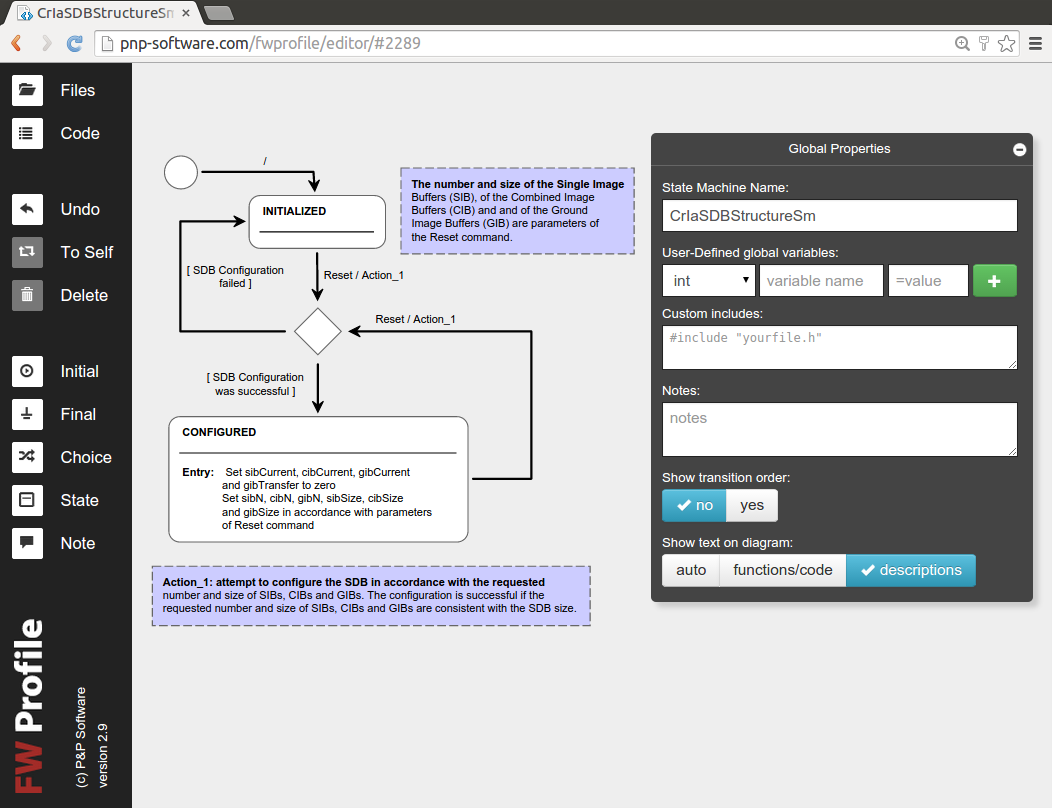
\includegraphics[scale=0.4,keepaspectratio=true]{FwProfileEditorScreenshot.png}
 \caption{Screenshot of the Framework Profile Editor}
 \label{fig:FwProfileEditorScreenshot}
\end{figure}

For each state machine or procedures, the FW Profile Editor offers two "views": the "description view" and the "code view". Users can change between the code view and the description view using a switch in the web-based interface of the editor (see box at the bottom of the "Global Properties" palette in figure \ref{fig:FwProfileEditorScreenshot}).

The two views are illustrated in figures \ref{fig:TsOutCmdSm} and \ref{fig:TsOutCmdSmCode} through the example of the OutCommand State Machine. The description view is used as a specification in the USP of the PUS Extension of the CORDET Framework (see reference [TsUsp]). The actions and guards of the state machine are described through a specification of what they should do. The code view associates code to the actions and guards in the state machine. The code may either take the form of a function name or it may consist of valid C code which directly implements the function. In the example of figure \ref{fig:TsOutCmdSmCode}, the former option. Thus, for instance, \texttt{OutCmdPendingEntry} is the name of a function which implements the entry action of state PENDING in the OutCommand State Machine.


\begin{figure}[H]
 \centering
 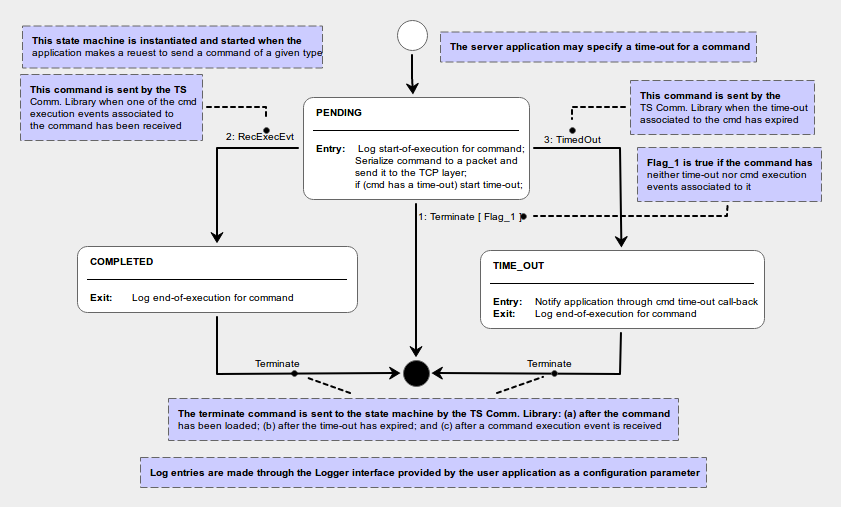
\includegraphics[scale=0.45,keepaspectratio=true]{TsOutCmdSm.png}
 \caption{Description View OutCommand State Machine}
 \label{fig:TsOutCmdSm}
\end{figure}


\begin{figure}[H]
 \centering
 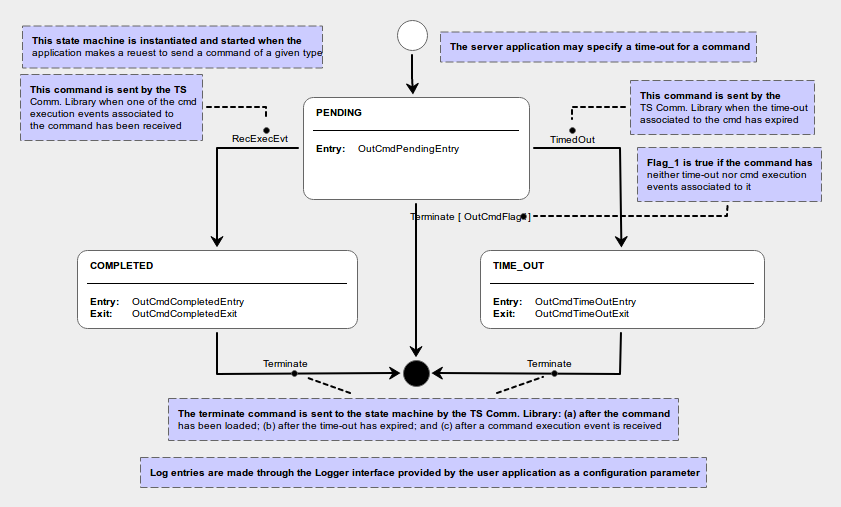
\includegraphics[scale=0.45,keepaspectratio=true]{TsOutCmdSmCode.png}
 \caption{Code View of OutCommand State Machine}
 \label{fig:TsOutCmdSmCode}
\end{figure}

%-----------------------------------------------------------------------------------------
\subsection{Generated Code}
The code generated by the FW Profile Tool for each state machine or procedure consists of three files:

\begin{itemize}
\item A header file which declares the following two items: 
\begin{enumerate}
\item The function to instantiate and configure the state machine or procedure, and
\item Any additional functions implementing actions or guards of the state machine or procedure. 
\end{enumerate}
\item A body file which implements the function which instantiates and configures the state machine or procedure.
\item A dummy \texttt{main} program which instantiates and configures the state machine or procedure and sends a few commands to it. This main program is only intended for demonstration/testing purposes and is not integrated with the application code. 
\end{itemize}

As noted in the previous section, the FW Profile Editor also gives users the option to define the implementation of an action or guard by directly entering the implementing code through the tool interface. In that case, the tool also generates a private (\texttt{static}) function with the code provided by the user. 

The code generated by the FW Profile Editor must be linked with the FW Profile Library (the necessary \texttt{\#include} statements are automatically generated). The library consists of a set of C modules which implement the behaviour of a generic state machine or procedure. Use of this library means that the code generated by the editor only needs to implement the configuration of a state machine or procedure (as opposed to implementing the state machine transition logic or the procedure execution logic). 

For state machines, the configuration code consists of a linear sequence of function calls which "build" the state machine by adding states and transitions and attaching them their attributes (the state and transition actions and the transition guards). Similarly, the configuration of a procedure consists of a sequence of function calls which build the procedure by adding nodes and control flows and to it and attaching them their attributes (the node actions and the control flow guards). 

%-----------------------------------------------------------------------------------------
\subsection{Use of Generated Code}
With the PUS Extension of the CORDET Framework, the auto-generated code is used to create and configure the state machines and procedures. The code must be linked with the manually written code of the PUS Extension of the CORDET Framework but does not need to manually modified in any way.  

The PUS Extension of the CORDET Framework code calls calls the \texttt{Create} function when it needs to instantiate a state machine or procedure. The \texttt{Create} function returns one instance of the state machine or procedure which is fully configured and ready to be used. No further interaction with the generated code is necessary.

%-----------------------------------------------------------------------------------------
\subsection{Summary of Mode of Use of FW Profile Editor}
The FW Profile Editor and its code generator are used as follows in the PUS Extension of the CORDET Framework:

\begin{fw_enumerate}
\item Specification of state machines and procedures using the "description view" of the FW Profile Editor. 
\item Definition of "code view" for the state machines and procedures within the FW Profile Editor. For each action or guard with non-default implementation, a function is defined and its name is entered in the tool. 
\item Generation of code using the FW Profile Editor code generator. For each state machine or procedure, two files are generated (one header file and one body file).
\item For each state machine or procedure, creation of a body file with the implementation of the functions implementing the non-default actions or guards of the state machine or procedure.
\end{fw_enumerate}




\end{document}